\documentclass[withoutpreface,bwprint]{cumcmthesis}
\usepackage{setspace}
\usepackage{makecell}
\usepackage{subcaption}

\title{基于LightGBM的电商需求预测模型}
\begin{document}

\begin{table}[]
  \centering % 让表格居中
  \begin{tabular}{|c|c|c|c|} % 使用 | 来添加边框
    \hline % 添加顶部横线
    \multicolumn{2}{|c|}{~~~~~队伍编号~~~~~} & \multicolumn{2}{|c|}{~~~~~MCB2301266~~~~~} \\
    \hline % 添加横线
    \multicolumn{2}{|c|}{赛道}   & \multicolumn{2}{|c|}{B} \\
    \hline % 添加底部横线
  \end{tabular}
\end{table}


   \maketitle
   \thispagestyle{empty}
\begin{abstract}
\begin{spacing}{1.5}
     \zihao{5}
     本文针对题目所提供四个数据集,研究并构建通过商家、商品和仓库多个特征参数来预测销售量的时间序列模型,期望对商家的销售和储存供应方面进行科学有效的预测和干预,来降低库存成本,同时保证商品的销售需求。

       在数据预处理方面,我们的团队对所有数据集和信息参数进行了综合概述。我们采用符合实际情况的正态分布模型对整体数据集进行了分析和筛选,同时利用\textbf{3-Sigma原则}和\textbf{Box-Cox标准化}方法对数据进行完善和剔除
     
     对于问题一,我们的团队参考了大量时间序列预测模型的文献,同时进行了进一步的实验比较,评估了各类时间序列预测模型的性能和算法效率。最终,我们选择了性能和算法效率均优秀的\textbf{LightGBM模型}。此外,我们结合\textbf{贝叶斯调参}对模型进行了进一步优化,以得到最终的训练模型。在验证集上,该模型的预测效果表现出高度精确性,其\textbf{1-wmape}的评估值为\textbf{0.534},并在准确率和效率综合得分上明显优于其他模型。对于商家、仓库和商品形成的时间序列,我们利用\textbf{K-Means算法}使用商品一级分类、商家分类、库存分类、商家规模、仓库类别、仓库区域、以及时间序列的平均值和方差等特征进行聚类分析,以确保相同类别的时间序列需求具有相似的特征。
     
     对于问题二,我们首先使用问题一的模型将附件5的数据进行聚类,将数据分成7个不同的类别,然后根据这些类别使用LightGBM算法进行预测。
     
     对于问题三,我们团队考虑规律性促销对预测结果的影响,通过引入0-1变量来描述该时间是否处于促销阶段,将附件6的数据设为1,附件1时间段设为0,由此预测6月份的促销阶段数据,通过训练我们的模型,其\textbf{1-wmape}的评估值为\textbf{0.5716}。

     我们团队使用了K-Means算法对相同特征的时间序列进行聚类,再使用LightGBM算法进行预测,相较于Arima算法1-wmape提升了10\%左右的精度,我们还考虑促销对预测的影响,通过引入变量提升模型预测精度。
     
\keywords{\quad LightGBM 算法 
          \quad K-Means算法
          \quad 贝叶斯优化
          \quad 时间序列预测
          }

\end{spacing}
\end{abstract}


%目录页
\thispagestyle{empty} % 目录页不显示页码
\tableofcontents 
\newpage

%正文
\setcounter{page}{0}
	\pagenumbering{arabic}
\section{问题的重述和分析}
    \subsection{问题重述}
    电商平台存在着上千个商家,他们将商品货物存放在电商配套的仓库。电商平台通过科学的管理手段和智能决策,利用大数据智能驱动的供应链来降低库存成本,同时保证商品的按时交付。在这一智能供应链中,预测扮演着关键的角色,它允许管理者提前了解各地的需求,从而使库存提前布置在靠近需求的仓库中。这里的预测任务主要是根据历史一段时间的需求量来预测各仓库中各商品的未来需求。这个被称为"预测维度",涵盖了不同商家在各仓库中存放的各种商品每天的数量。通常情况下,企业会首先根据数据的历史情况,分析需求量序列的数理特征,对相似的需求量序列进行分类,并根据分类结果实现更加精准的预测。这种供应链的优化旨在实现高效的库存管理和交付流程,从而提高整体业务效益。
    
    附件1提供了电商零售商家过去6个月内在不同电商仓库中的商品每日出货量的历史记录。本题假定这些出货量即为历史上各商品在不同仓库中的需求量。此外,附件2\~{}4提供了有关各商品、商家和仓库的信息,包括分类、品牌、生效日期等。引入这些信息有助于更精确地进行库存预测和供应链管理。这些数据将为解决以下三个问题提供关键支持:
    
    问题1:使用附件1\~{}4的数据,建立一个模型,预测2023年5月16日至2023年5月30日期间各商家在各仓库的商品需求量。此外,讨论如何将这些时间序列分类,以便将相似需求特征的序列划分为一类。
    
    问题2:讨论附件5中新出现的商家+仓库+商品维度的原因,可能由于新上市商品或仓库变动。使用历史附件1中的数据,找到与新维度相似的序列,然后预测这些新维度在2023年5月16日至2023年5月30日期间的需求。
     
    问题3:每年6月会出现规律性的大型促销,这给需求量的精准预测和履约带来了挑战。附件6提供了去年双十一期间的商家+仓库+商品维度的需求数据。请参考这些数据,预测2023年6月1日至2023年6月20日期间的需求。
    
    \subsection{问题分析}
    首先,要对于数据集进行预处理,综合概述所有数据集和信息参数。采用符合问题实际要求的方法对数据进行分析、筛选和完善,以准备数据用于建模。

     针对问题一,研究了各种时间序列预测模型,并选择合适的模型,调参来进一步优化模型。另外,对商家、仓库和商品的时间序列进行分类,确保相同类别的时间序列需求具有相似特征。

     针对问题二,在问题一的模型基础上,结合附件5的数据中新出现的商家+仓库+商品维度,进一步优化预测模型。

     针对问题三,考虑了规律性促销对预测结果的影响。引入0-1变量以描述促销阶段,进一步优化预测模型。
     
    \section{模型假设和数据预处理}
    \subsection{模型假设}

    \subsection{数据探索}
    附件1包含了过去六个月内不同仓库和商家销售商品的每日销售数据。附件2涵盖了商品的三级分类信息,使我们能够更好地理解不同商品的性质。附件3提供了有关不同商家主要营销商品的分类和销售规模信息,从而揭示了商家的经营策略。附件4包含了有关不同仓库的类别和地理位置数据,这对于分析物流和库存管理至关重要。我们团队使用了Pandas库和spsspro,通过对这些附件的数据进行初步分析,创建了信息图表,以便更全面地理解和解释数据的内在关系。

    通过分析附件2的商品分类数据桑基图\ref{附件2商品分类桑基图},我们明显地发现,在这2302件商品中,家装建材类别占据了主导地位。
    \begin{figure}[htbp]
     \centering
     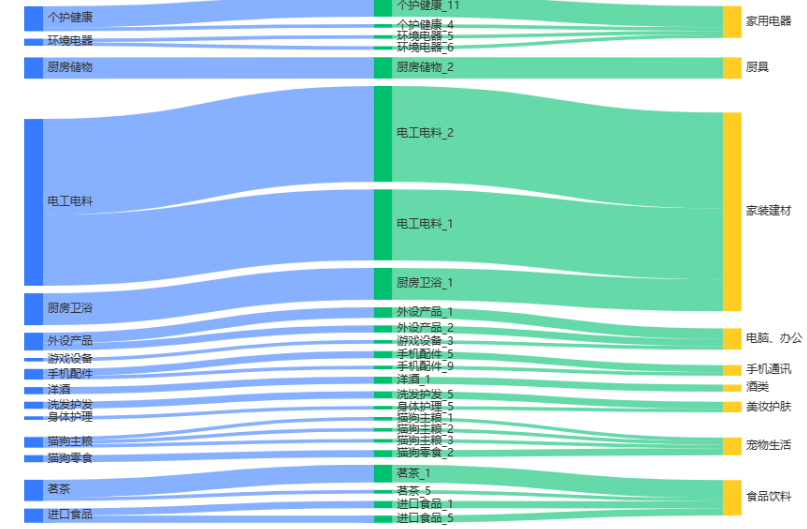
\includegraphics[width=15cm,height=9cm]{figure/附件2数据分析2.png}%figure目录存放图片
     \caption{附件2商品分类桑基图}
     \label{附件2商品分类桑基图}
    \end{figure}

      通过分析附件3的数据桑基图\ref{附件3数据分析桑基图},我们明显地发现商家们主要销售家用电器、食品饮料、电脑办公、家居日用、手机通讯、美妆护肤和家装建材等商品。与此同时,这些商品的库存分类主要集中在B级别,而绝大多数商家的规模被归为Large。
    \begin{figure}[htbp]
     \centering
     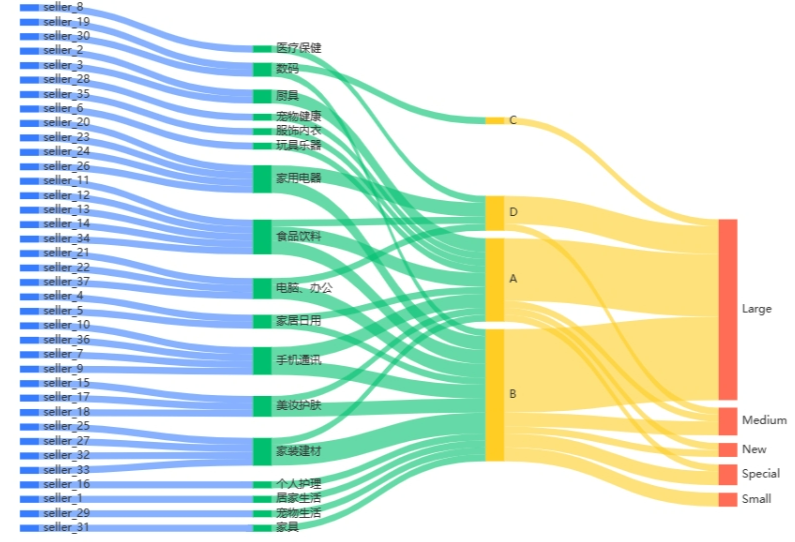
\includegraphics[width=15cm,height=9cm]{figure/附件3数据分析桑基图.png}%figure目录存放图片
     \caption{附件3数据分析桑基图}
     \label{附件3数据分析桑基图}
    \end{figure}

      通过对附件4的数据金字塔图\ref{附件4数据分析金字塔图}进行分析,明显可见,仓库主要以区域仓为主,并且大多数位于华东、华北、华南、华中和西南这五大区域。区域仓和中心仓是仓储管理中常用的两种不同类型的仓库。
      
      区域仓通常位于市场或客户需求密集的地区。主要功能是为特定地理区域提供产品供应,以满足该地区的需求。区域仓库通常存储相对较小数量的产品,并通常用于快速配送和满足地方市场的需求。
      
      中心仓通常位于一个中心地理位置,通常是国家或地区的中心,以便更好地服务整个市场。主要功能是集中存储大量产品,通常用于分配给不同的区域仓库或零售店铺。中心仓通常拥有更大的存储容量,用于批量分拨和补充区域仓库的库存。
    \begin{figure}[htbp]
     \centering
     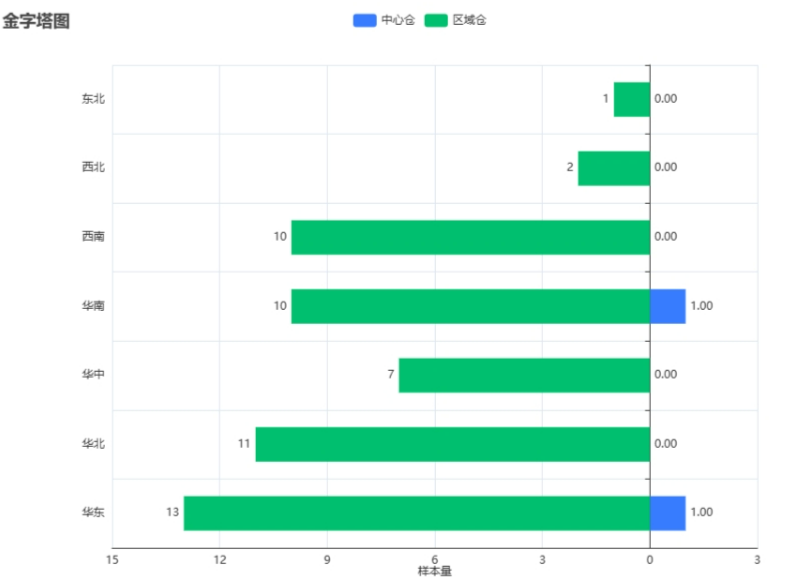
\includegraphics[width=15cm,height=9cm]{figure/附件4数据分析金字塔图.png}%figure目录存放图片
     \caption{附件4数据分析金字塔图}
     \label{附件4数据分析金字塔图}
    \end{figure}

\subsection{数据预处理}
    在上述四个附件的数据分析的基础上,我们团队通过python中的pandas库分别对附件1,2,3,4进行读取,对数据进行以下处理:
    
    $\bullet$剔除异常数据
    
      一般而言,噪声值对机器学习会有较大的影响,对于某些特定分布的数据集,机器学习的拟合效果好。因此,我们选用常见的正态分布处理数据,使用3-Sigma原则去除数据集异常值,因为这些数据发生概率小,可能由于某店铺推出促销活动,当天出现极端天气导致商品滞销等不可预测因素的影响。若数据服从正态分布,则若$P(|x - \mu| > 3\sigma) \leq 0.003$,则x被认为是异常值,若数据不满足正态分布,如\ref{部分出货量分布},我们使用Box-Cox标准化:$$y(\lambda) = \begin{cases}\frac{
      y^\lambda - 1}{\lambda} & \lambda \neq 0 \\
      lny & \lambda = 0
\end{cases}$$
将数据转换成正态分布,如\ref{BOX-COX标准后出货量分布}为转换后的分布,转换后满足正态分布再使用3-Sigma剔除异常值。
    \begin{figure}[htbp]
      \centering
        \begin{subfigure}{0.4\textwidth}
          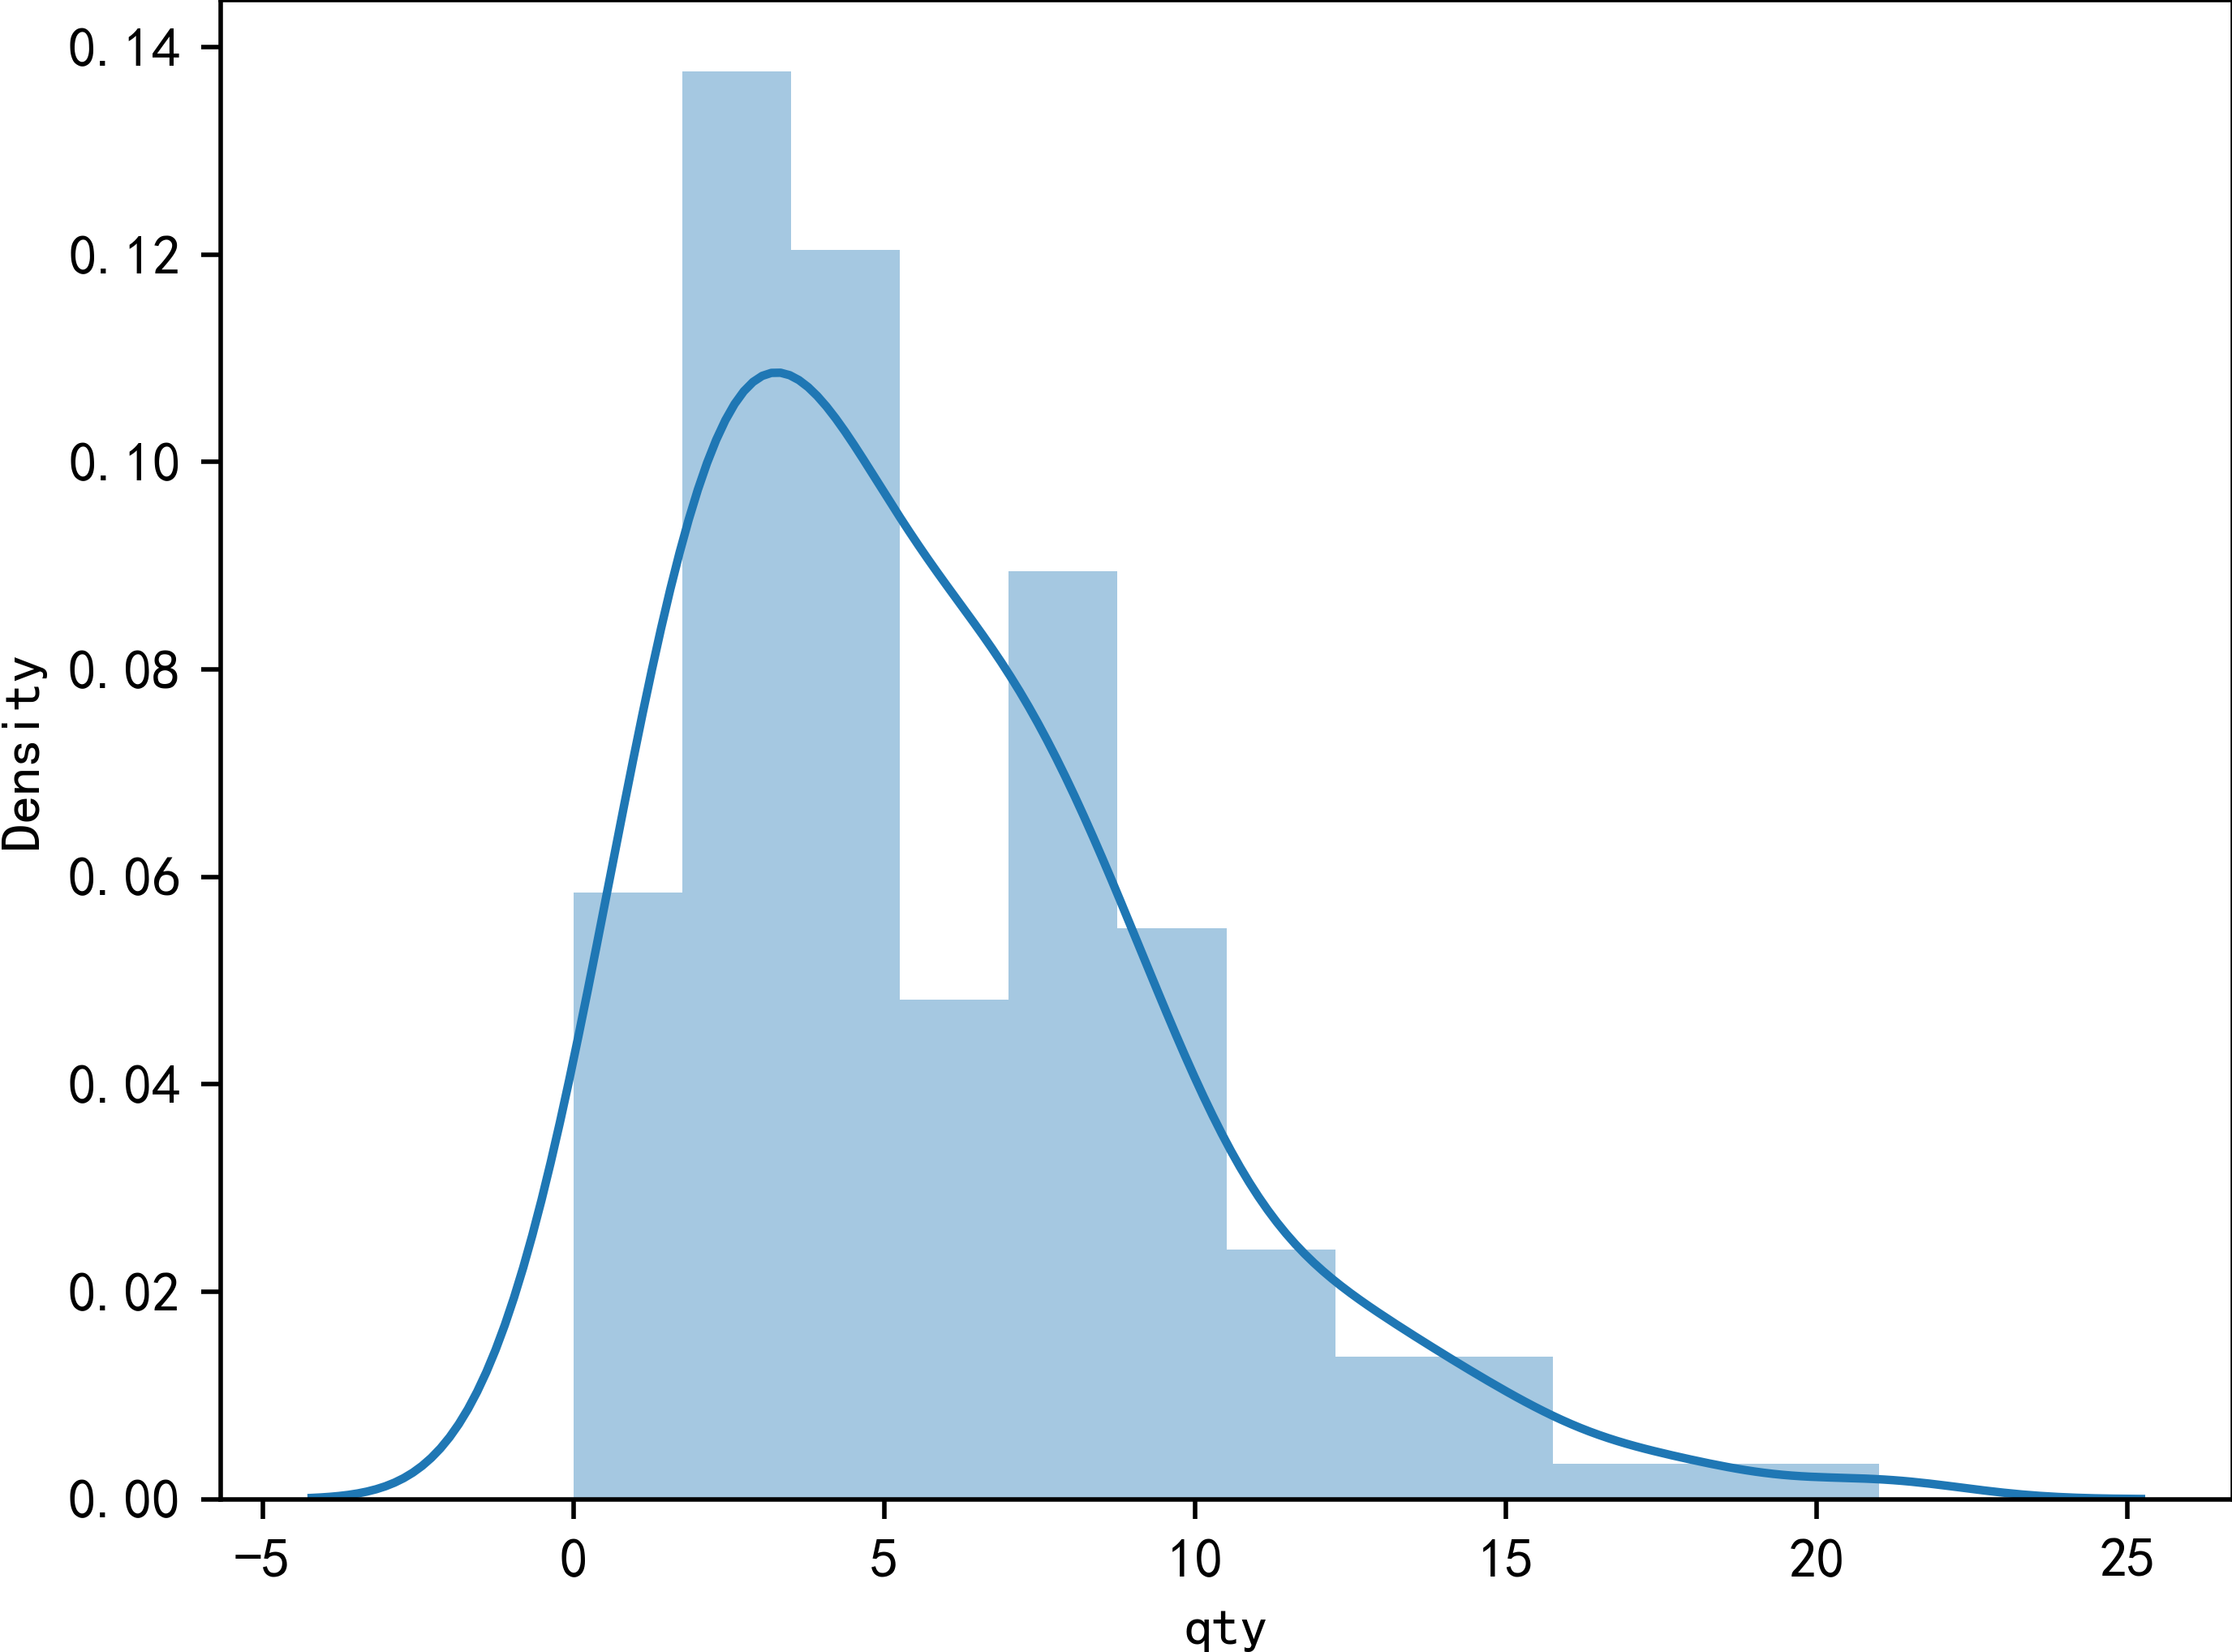
\includegraphics[width=\textwidth]{figure/qty分布.png}
          \caption{部分出货量分布}
          \label{部分出货量分布}
        \end{subfigure}
        \begin{subfigure}{0.4\textwidth}
          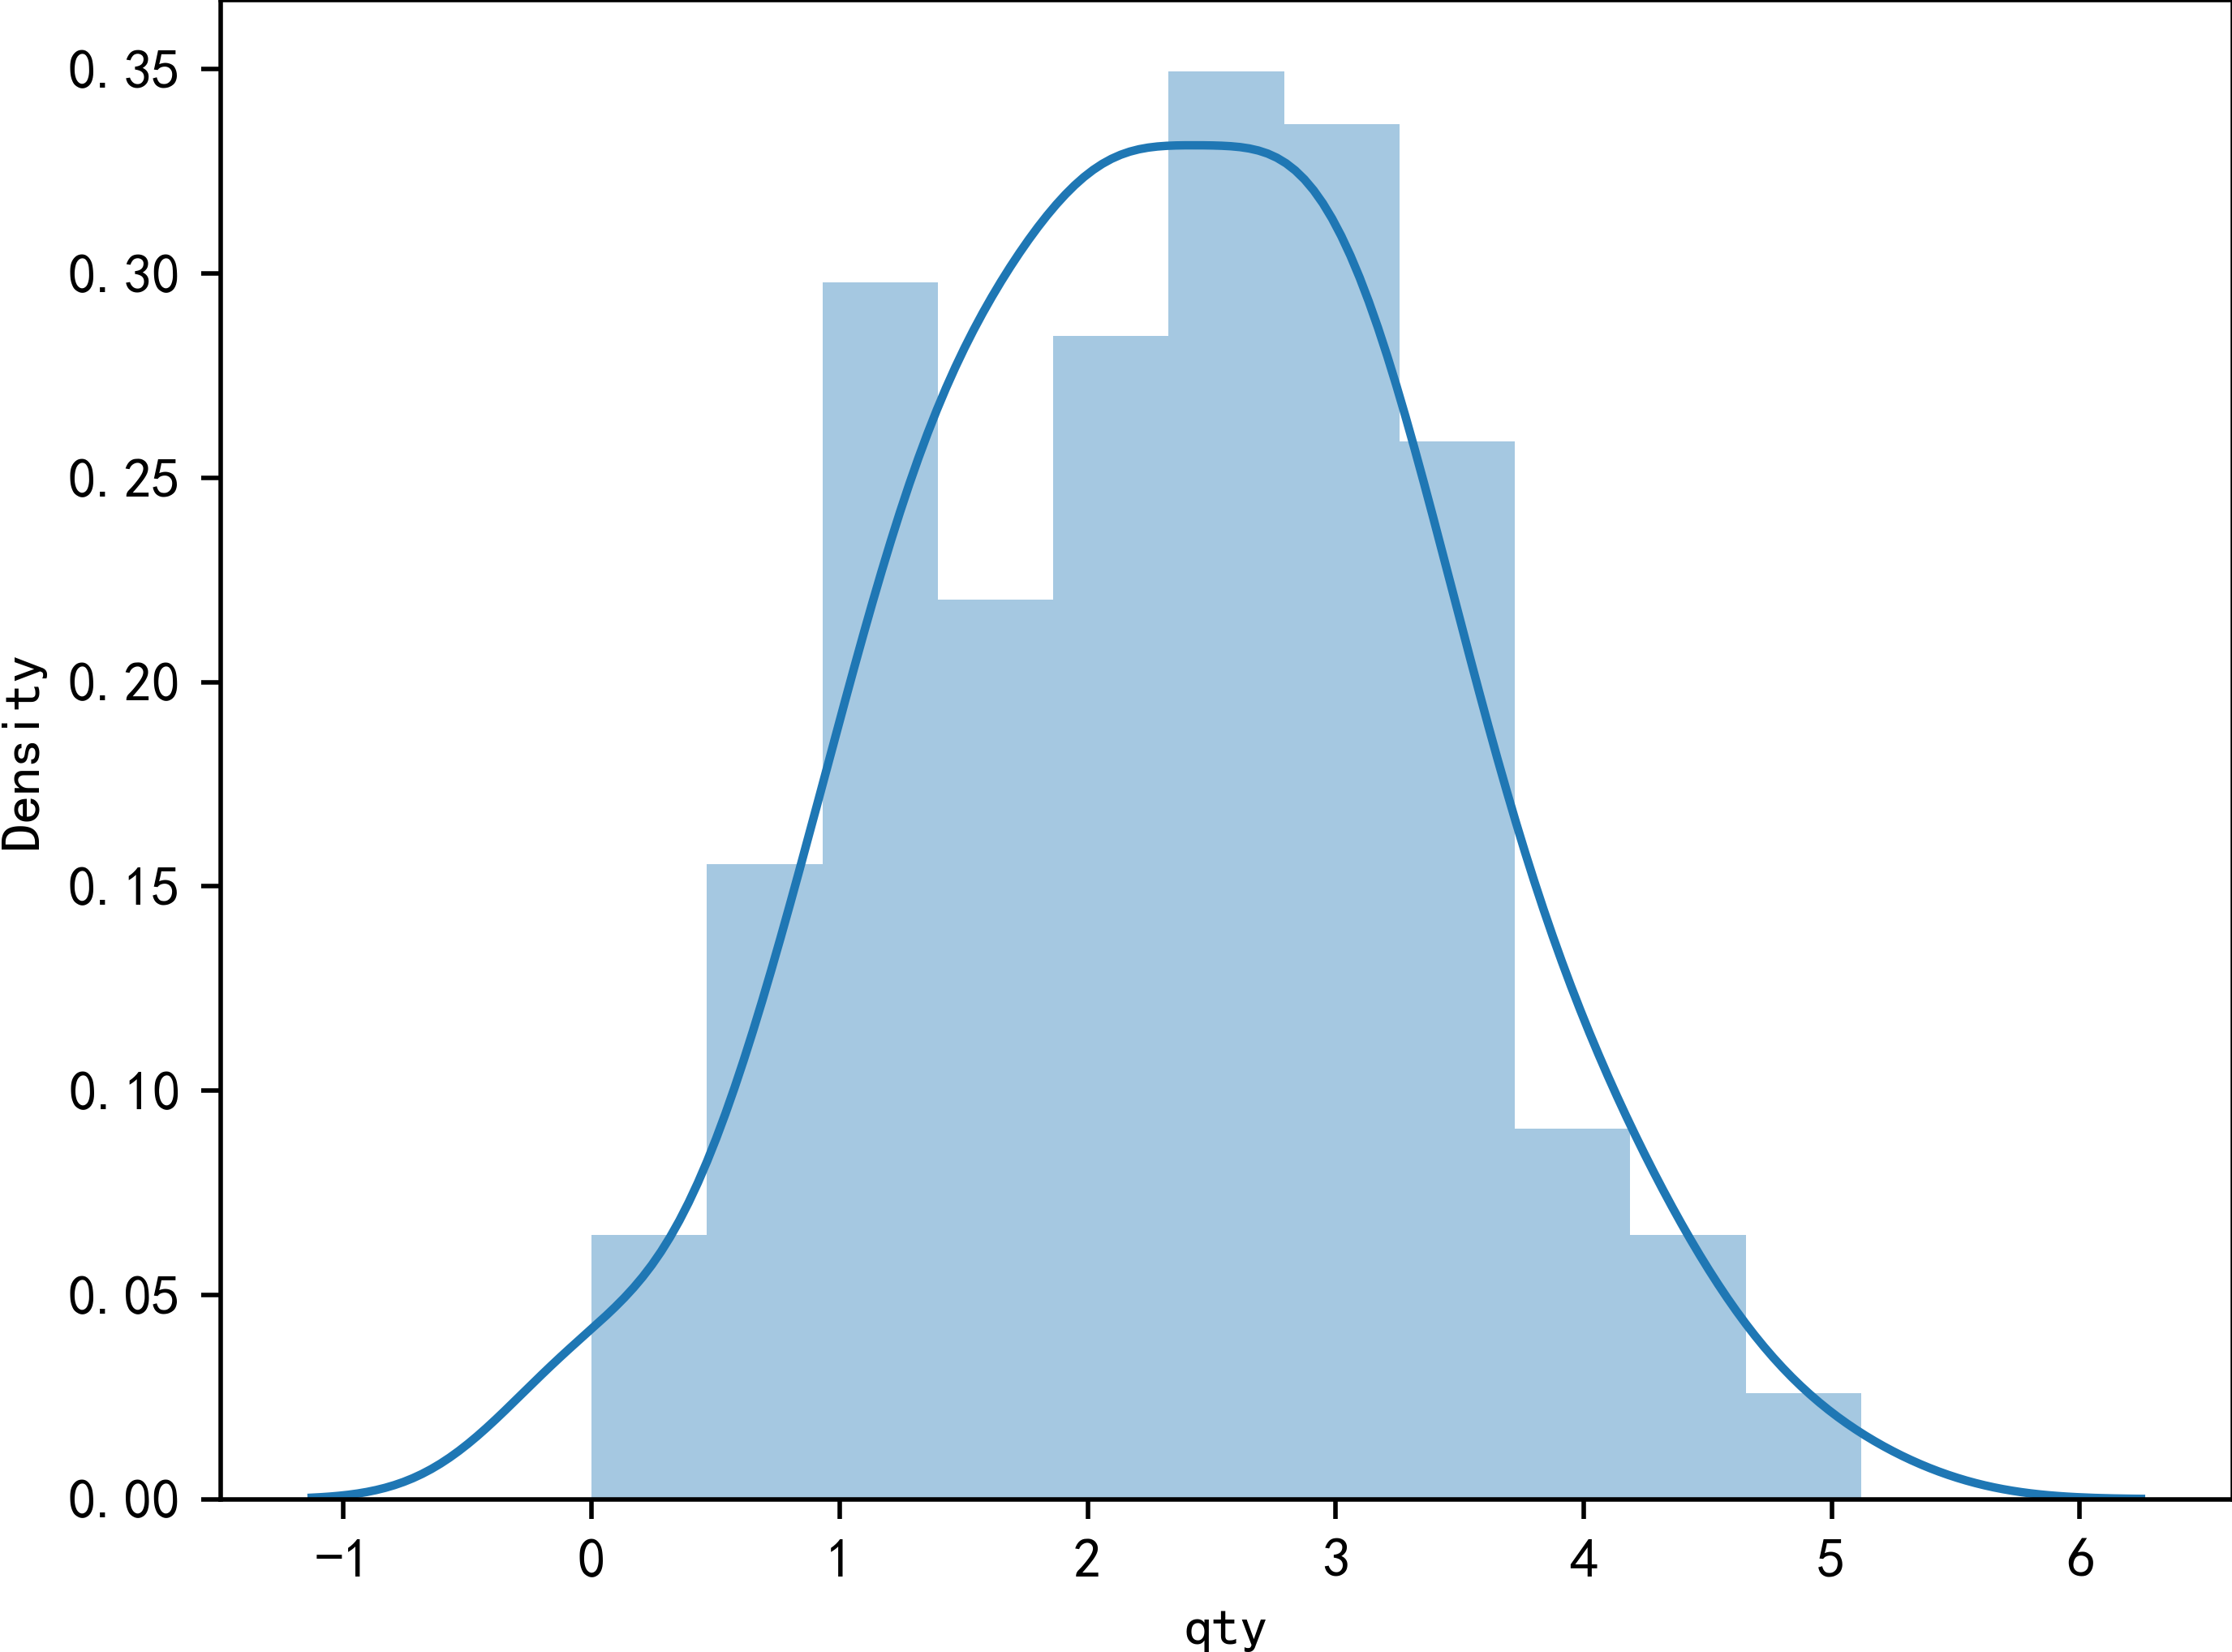
\includegraphics[width=\textwidth]{figure/qty分布BOXCOX转换.png}
          \caption{BOX-COX标准后出货量分布}
          \label{BOX-COX标准后出货量分布}
        \end{subfigure}
    \end{figure}
\subsection{特征工程}
     完成对数据的预处理以后,接下来是对数据集进行特征工程:
    \begin{enumerate}
    \item 将商家,商品,仓库信息的类别特征进行独热编码。这将使每个类别特征的每个类别都成为新的二进制列。在后续的预测模型的构建中,让我们在简单的时间序列模型的基础上能够综合更多的商品信息,以便有更加精准的预测结果。
    \item 时间序列滚动窗口处理
    
   \qquad 机器学习方法处理时序问题的基本思路:把时序切分成一段历史训练窗口和未来的预测窗口,对于预测窗口中的每一条样本,基于训练窗口的信息来构建特征,转化为一个表格类预测问题来求解。

   \qquad 一般我们需要确定几个参数:
    
    \qquad 1)历史窗口的大小,即预测未来时,要参考过去多少时间的信息作为输入。经过尝试,我们选择以30天作为历史窗口,揭示了数据集按月的周期性变化。
    
    \qquad 2)预测点 gap 的大小,即预测未来时,我们是从何时开始预测。我们根据实际需求,选择$x_{k+1}$为预测起点。
    
   \qquad 3)预测窗口的大小,即需要连续预测多长的未来值。为了更好的揭示以月为周期的变化规律,并且考虑到预测过长时间时,结果的不准确性提高。经过一系列测试以后,我们选择14天作为预测窗口的大小。

    \qquad 首先,利用历史窗口这部分的信息输入构建特征,再去预测预测窗口中的值,计算与实际数据集之间的误差,再不断迭代改进。这个窗口不断往前滑动,形成多个预测窗口的样本。
    
    \qquad 实现步骤如\ref{时间窗口处理},建立时间预测滚动窗口一定程度上可以提高数据利用率,提高模型准确度。
    \begin{figure}[htbp]
       \centering
       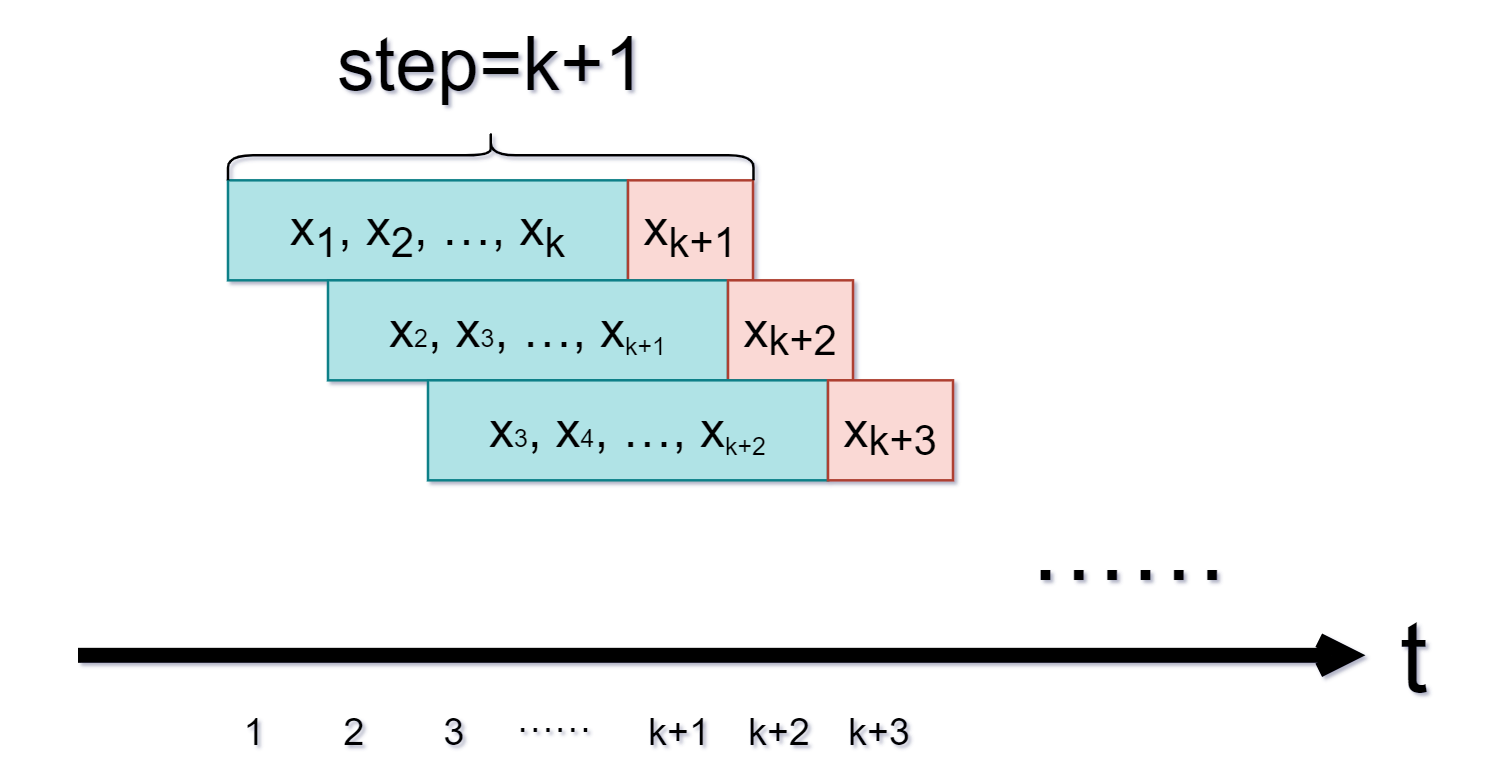
\includegraphics[width=10cm,height=5cm]{figure/时间窗口.png}%figure目录存放图片
       \caption{时间序列窗口滚动处理}
       \label{时间窗口处理}
    \end{figure}
    \end{enumerate}

\section{模型的建立和求解}
\subsection{问题一的建模和求解}
\subsubsection{模型的建立}
    问题1的要求是基于附件1中不同电商仓库的商品每日出货量历史记录,建立时间序列的预测模型并构建时间序列的分类模型,以便将具有相似需求特征的时间序列分为不同类别。
    
    对于商品的时间序列预测方法,有许多主要的方法可供选择,其中包括指数平滑法、神经网络、遗传算法、ARIMA算法、回归算法以及其他一些方法。

    研究表明,ARIMA模型在处理具有季节性变化的时间序列数据时表现出色。例如,姜向荣\textsuperscript{\cite{a}}将ARIMA算法应用于具有季节性变化的时间序列,取得了良好的预测性能。此外,一些研究人员\textsuperscript{\cite{b},\cite{c},\cite{d}}还将ARIMA模型与节假日相关性、卡尔曼滤波器和其他算法相结合,以提高模型的性能和算法效率,从而在实际应用中取得了良好的效果。

    在M5 accuracy competition的比赛中,大多数被检查的方法都使用了LightGBM,这是一种使用梯度增强树进行非线性回归的ML算法。LightGBM在预测任务中比其他ML替代方案显示出一些优势,比如M5 Accuracy竞赛所考虑的,因为它允许有效处理各种类型(数字、二进制和分类)的多个特征(例如,过去的销售和外生/解释变量),与典型的梯度增强(GBM)实现相比计算速度快,不依赖于数据预处理和转换,并且只需要优化相对少量的参数(例如,学习率、迭代次数、将特征值放入桶中的最大仓数、估计器数量和损失函数)。在这方面,LightGBM非常方便地实验和开发解决方案,这些解决方案可以准确地推广到显示互相关的大量序列。事实上,LightGBM可以被认为是Kaggle最近预测比赛中的标准选择方法,并且在Kaggle上发布的M5 Accuracy比赛的讨论和笔记本集中在LightGBM的实现和这种方法的变体上。\textsuperscript{\cite{e}}故在模型上我们团队选择LightGBM来进行第一问的求解。
    
\subsubsection{模型的求解}
     \subsubsection*{(1) K-Means聚类}

$\bullet$特征提取与选择

   为了使滑动窗口效果更好,并以此提高模型精确度,我们采用时序值衍生的滑动窗口统计作为特征并结合已有数据集的属性和特征进行聚类,以达到更好的聚类效果。

   具体操作即使用先前时间观察值的统计信息作为特征。比如对于t时刻,取前30天的统计值作为特征,也就是将t-1$\sim$t-31这个时间段数据的平均数、中位数、标准差、最大值、最小值等作为特征,此时指定的窗口就是30。再通过对特征重要性的排序,我们最后选择平均值和方差,作为K-Means聚类的聚类特征。

$\bullet$K-Means聚类

     K—Means基本思想是,通过迭代寻找K个簇(Cluster)的一种划分方案,使得聚类结果对应的损失函数最小。其中,损失函数可以定义为各个样本距离所属簇中心点的误差平方和:

     $$J(c,\mu)=\sum_{i=1}^M ||x_i-\mu_{c_i}||^2$$

     其中$x_i$代表第$i$个样本,$c_i$是$x_i$所属的簇,$\mu_{c_i}$代表簇对应的中心点,M是样本总数。

     具体步骤:

     1)随机选取k个中心,记为$\mu_1^{(0)} , \mu_2^{0} , \dots, \mu_k^{0}$

     2)令t=0,1,2,$\dots$为迭代步数,重复如下过程直到J收敛:

     对于每一个样本$x_i$,将其分配到距离最近的中心

     $$c_i^t = -argmin_k ||x_i-\mu_k^t||^2$$

     对于每一个类中心k,重新计算该类的中心:

     $$\mu_k^{t+1} = -argmin_{\mu}  \sum_{i:c_i^t=k}^k ||x_i-\mu||^2$$

    $\bullet$聚类结果分析
   
   我们通过肘部图寻找最合适的分类个数。根据聚合系数折线图\ref{肘部图}可知,当类别数为7时,折线的下降趋势趋缓,故可将类别数设定为7。
   
   
    \begin{figure}[htbp]
     \centering
     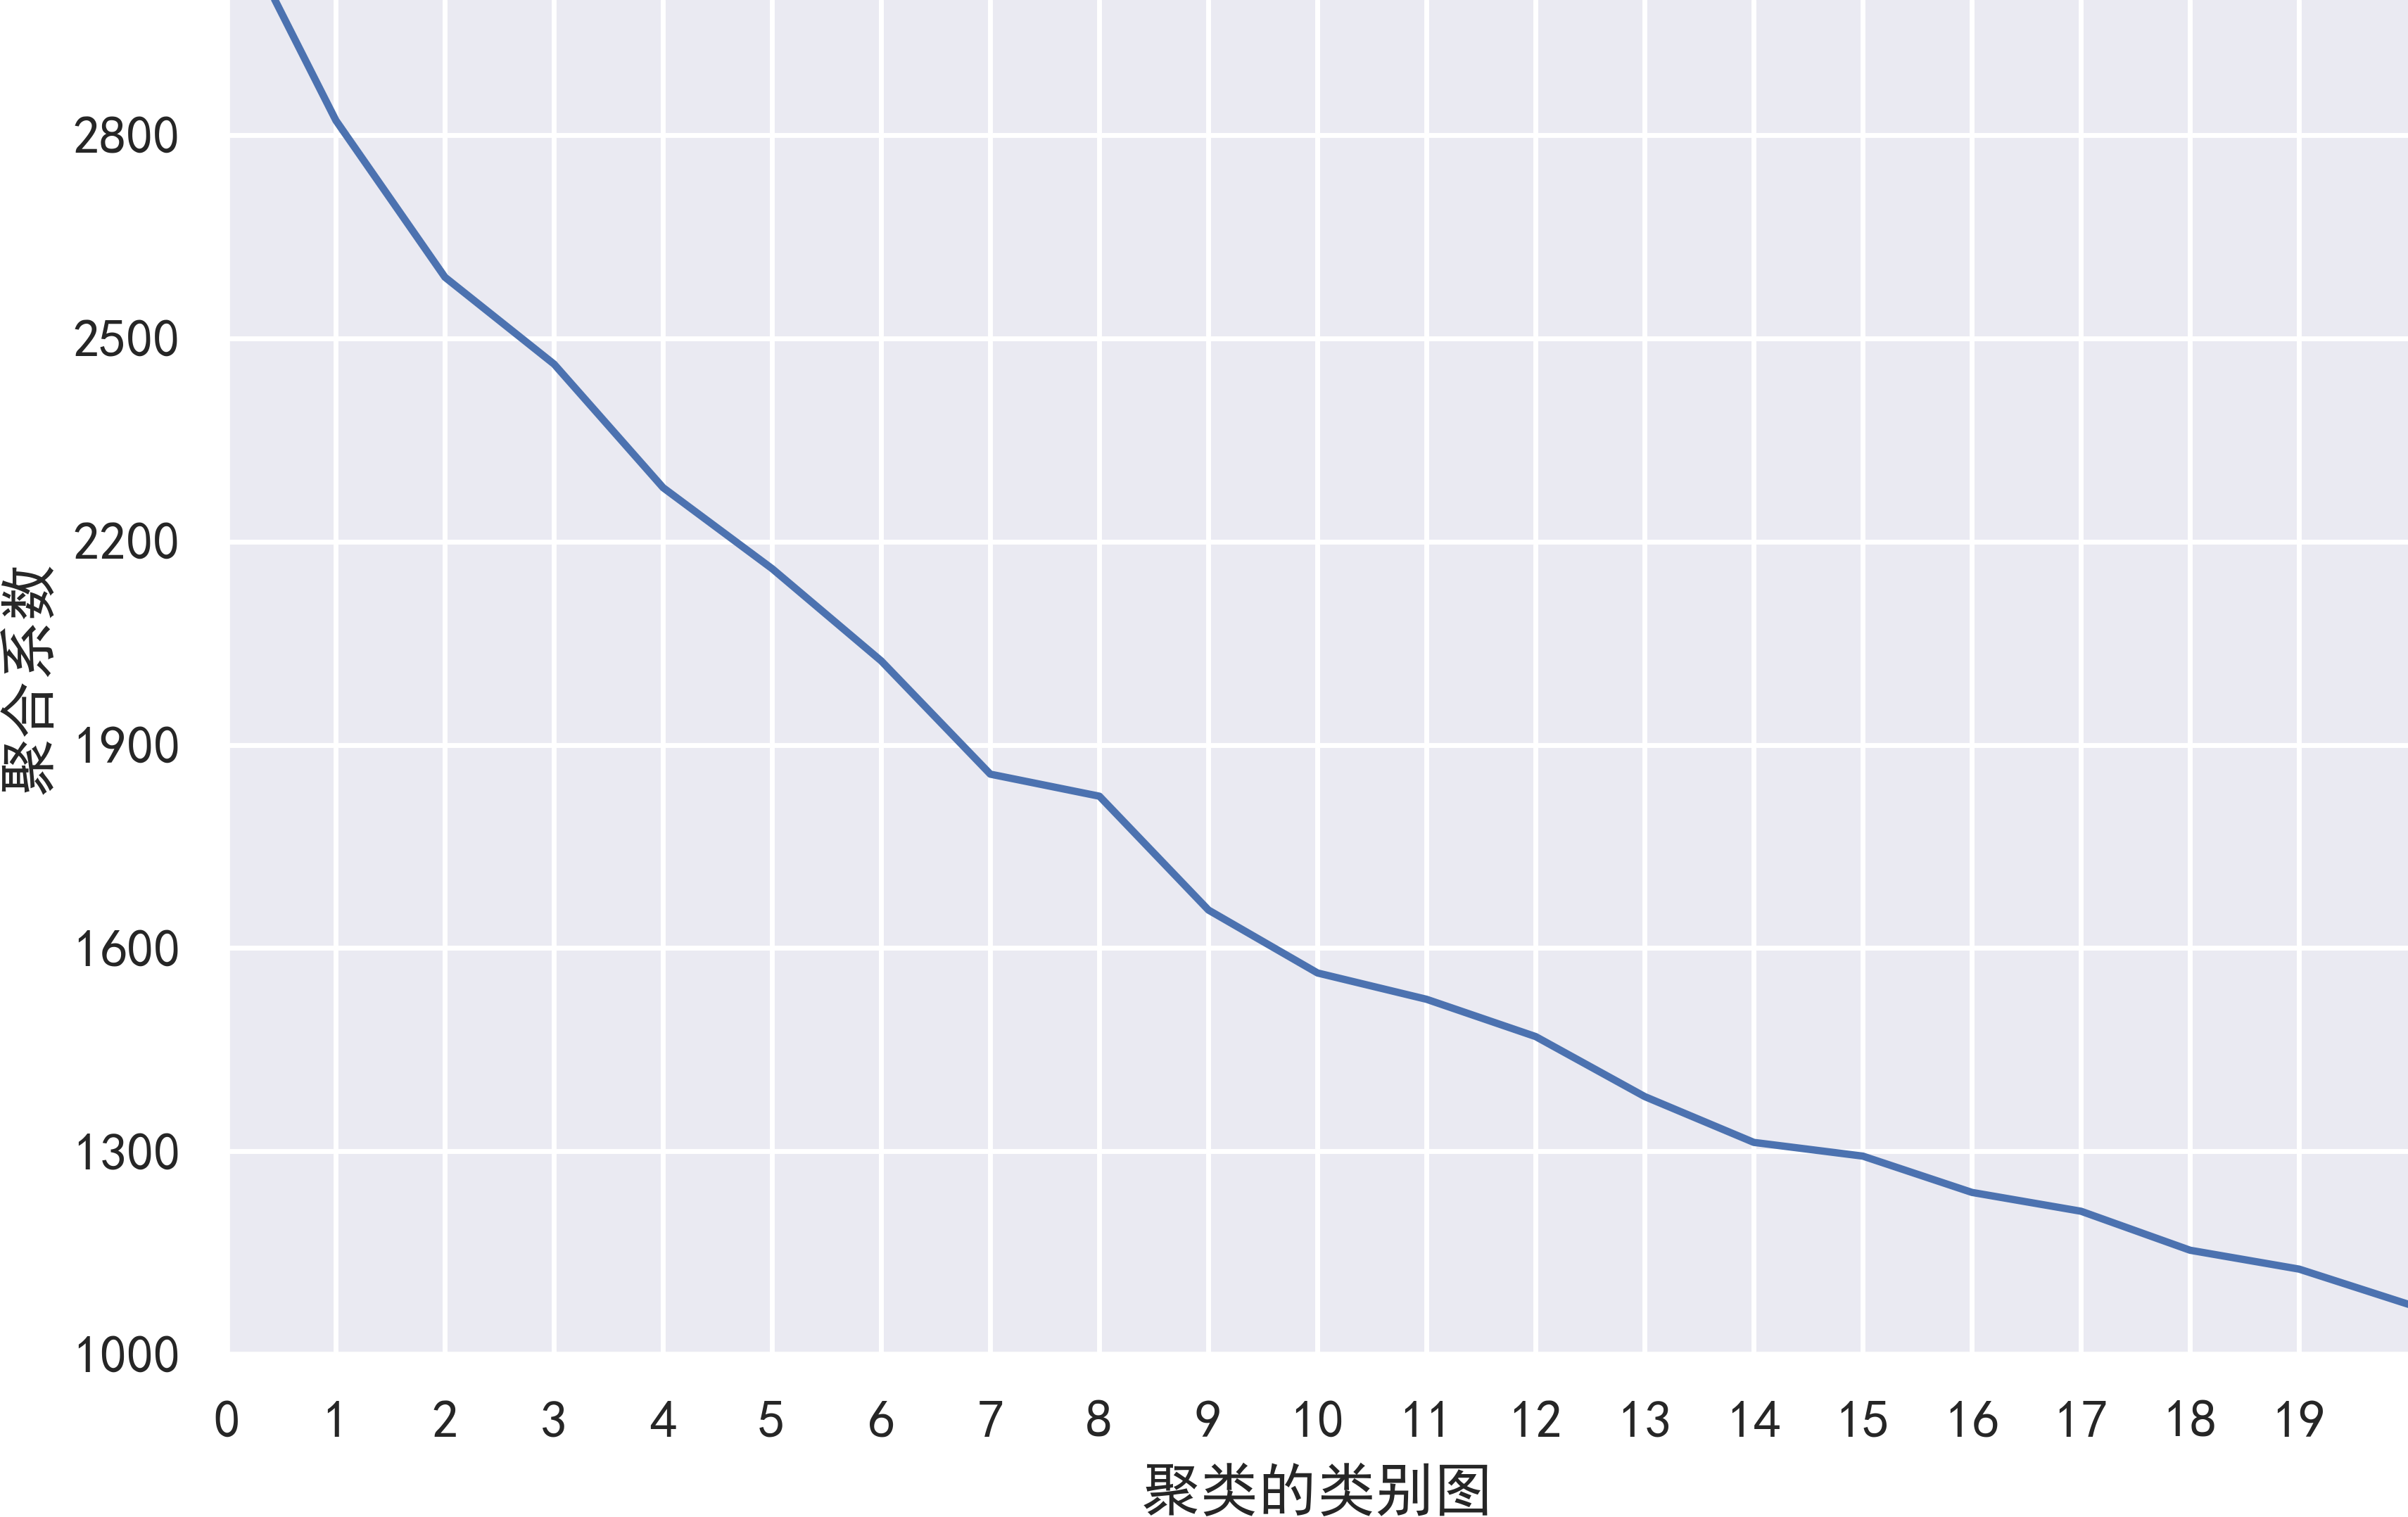
\includegraphics[width=15cm,height=9cm]{figure/肘部图.png}%figure目录存放图片
     \caption{肘部图}
     \label{肘部图}
    \end{figure}
    
    通过K-Means算法我们把时间序列分成7类,7类数量占比如图\ref{Kmeans分类类别},通过分析聚类结果,我们得到“特别商家,电脑,办公,华东发货”, “大商家,食品饮料,华东发货”, “大商家,食品饮料,华北发货”, “大商家,食品饮料,华南发货”, “大商家,家装建材,华东发货”, “大商家,食品饮料,西南发货”, “宠物,华中发货”,我们发现“特别商家,电脑,办公,华东发货”类别标准差较小,说明该类时间序列数据较接近平均值,“大商家,食品饮料,华东发货”类别标准差较大,时间序列不接近平均值等等,由此说明该聚类可以很好把该时间聚类的特征分类。
    \begin{figure}[htbp]
     \centering
     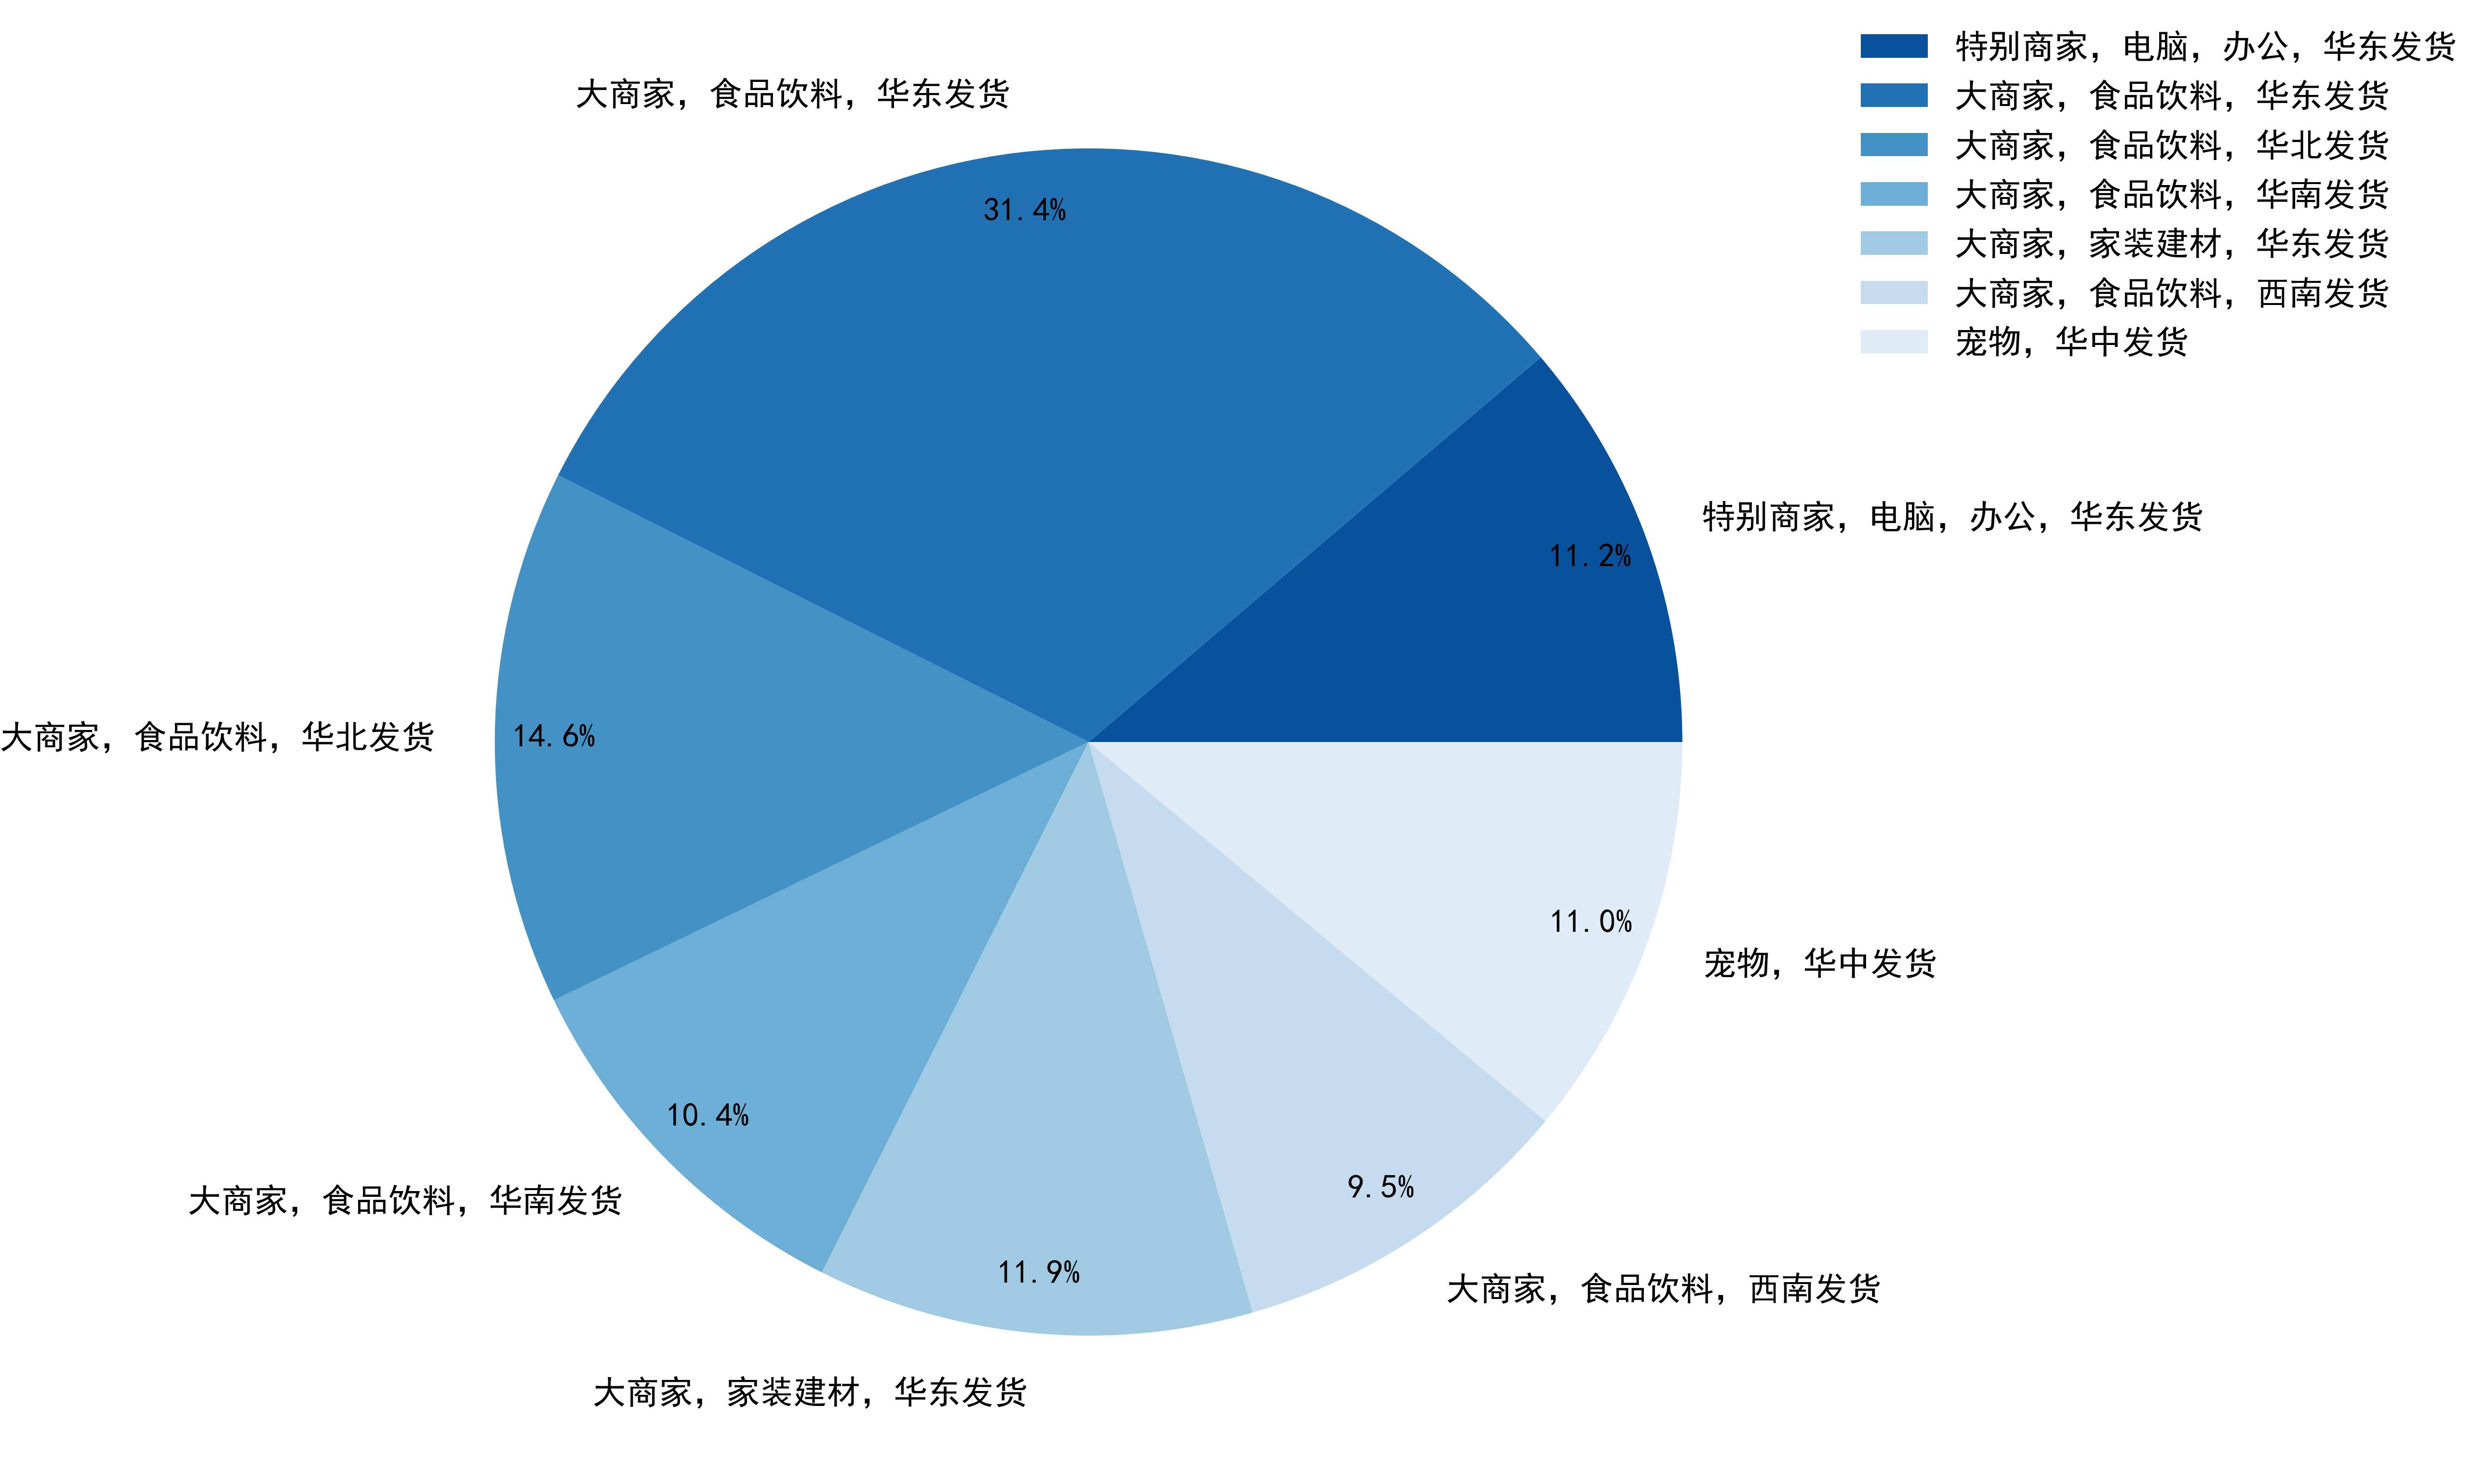
\includegraphics[width=15cm,height=9cm]{figure/Kmeans分类类别比例.png}%figure目录存放图片
     \caption{Kmeans分类类别}
     \label{Kmeans分类类别}
    \end{figure}
    \newpage

\subsubsection*{(2) 预测模型对比}
$\bullet$LightGBM模型

    GBDT (Gradient Boosting Decision Tree) 其主要思想是利用弱分类器(决策树)迭代训练以得到最优模型。LightGBM在传统的GBDT基础上引入了两个新技术:梯度单边采样(Gradient-based One-Side Sampling,GOSS)和独立特征合并(Exclusive Freature Bundling EFB)。LightGBM具有不易过拟合,高效且具有良好准确性,特别适用于处理大规模数据集等优点。
    
    GOSS 对小梯度样本点进行随机采样,保留对信息增益影响更大的梯度大的样本,在保持信息增益评估的精度前提下,大大提高了模型学习速率,且在采样率相同情况下,梯度单边采样的结果比随机采样准确率更高。EFR则实现了互斥特征的捆绑,达到减少特征维度的目的,提高了模型运算效率。另外,相较于传统GBDT算法使用了pre-sorted算法以精确分割数据,LightGBM使用了直方图算法,即将连续浮动的特征离散成k个离散值,并构造宽度为k的直方图,大大降低了内存消耗以及数据分割复杂度。对于给定数据集:$D=\lbrace(X_i,Y_i),i=1,2,3\dots,n,X_i\in R,Y_i\in R\rbrace$,其中,n为样本个数,每个样本有P个特征。给定损失函数$L(y,f(x))$,输出回归树$f(x)$,具体算法步骤如下:

    初始化$f_0(x)$,即
  $$f_0(x)=arg\quad\min\nolimits_{\theta}\sum_{i=1}^{N}L(y_i,\theta)$$
    计算损失函数的负梯度作为残差估计,即
    $$r_{im}=-[\frac{\partial L(y_i,f(x_i))}{\partial f(x_i)}]_{f(x)=f_{m-1}(x)}  (i=1,2,\dots,N)$$
    拟合残差树,计算损失函数最小值,即
    $$\gamma_{jm}=arg\quad\min\nolimits_{\gamma} \sum\limits_{x_i \epsilon R_{jm}} L(y_i,f_{m-1}(x_i)+\gamma)$$
    更新回归树,即
    $$f_m(x)=f_{m-1}(x)+\sum\limits_{j=1}^{J_m}\gamma_{jm}I,x\epsilon R_{jm}$$
    由此得到最终的$f(x)$。

     对于时间序列预测,我们使用Arima,Prophet,线性回归,LightGBM,LSTM模型做对比,我们用1-wmape做指标,寻找预测效果最好的模型。由\ref{模型对比}可见,传统时间预测模型如Arima,Prophet,预测结果甚至不如简单的直线拟合。深度学习模型LSTM虽然比机器学习模型lightgbm预测效果好,但是LSTM运行较为耗时且提升不是很大,因此接下来的预测我们使用lightgbm进行时间序列预测。
      
     \begin{figure}[htbp]
     \centering
     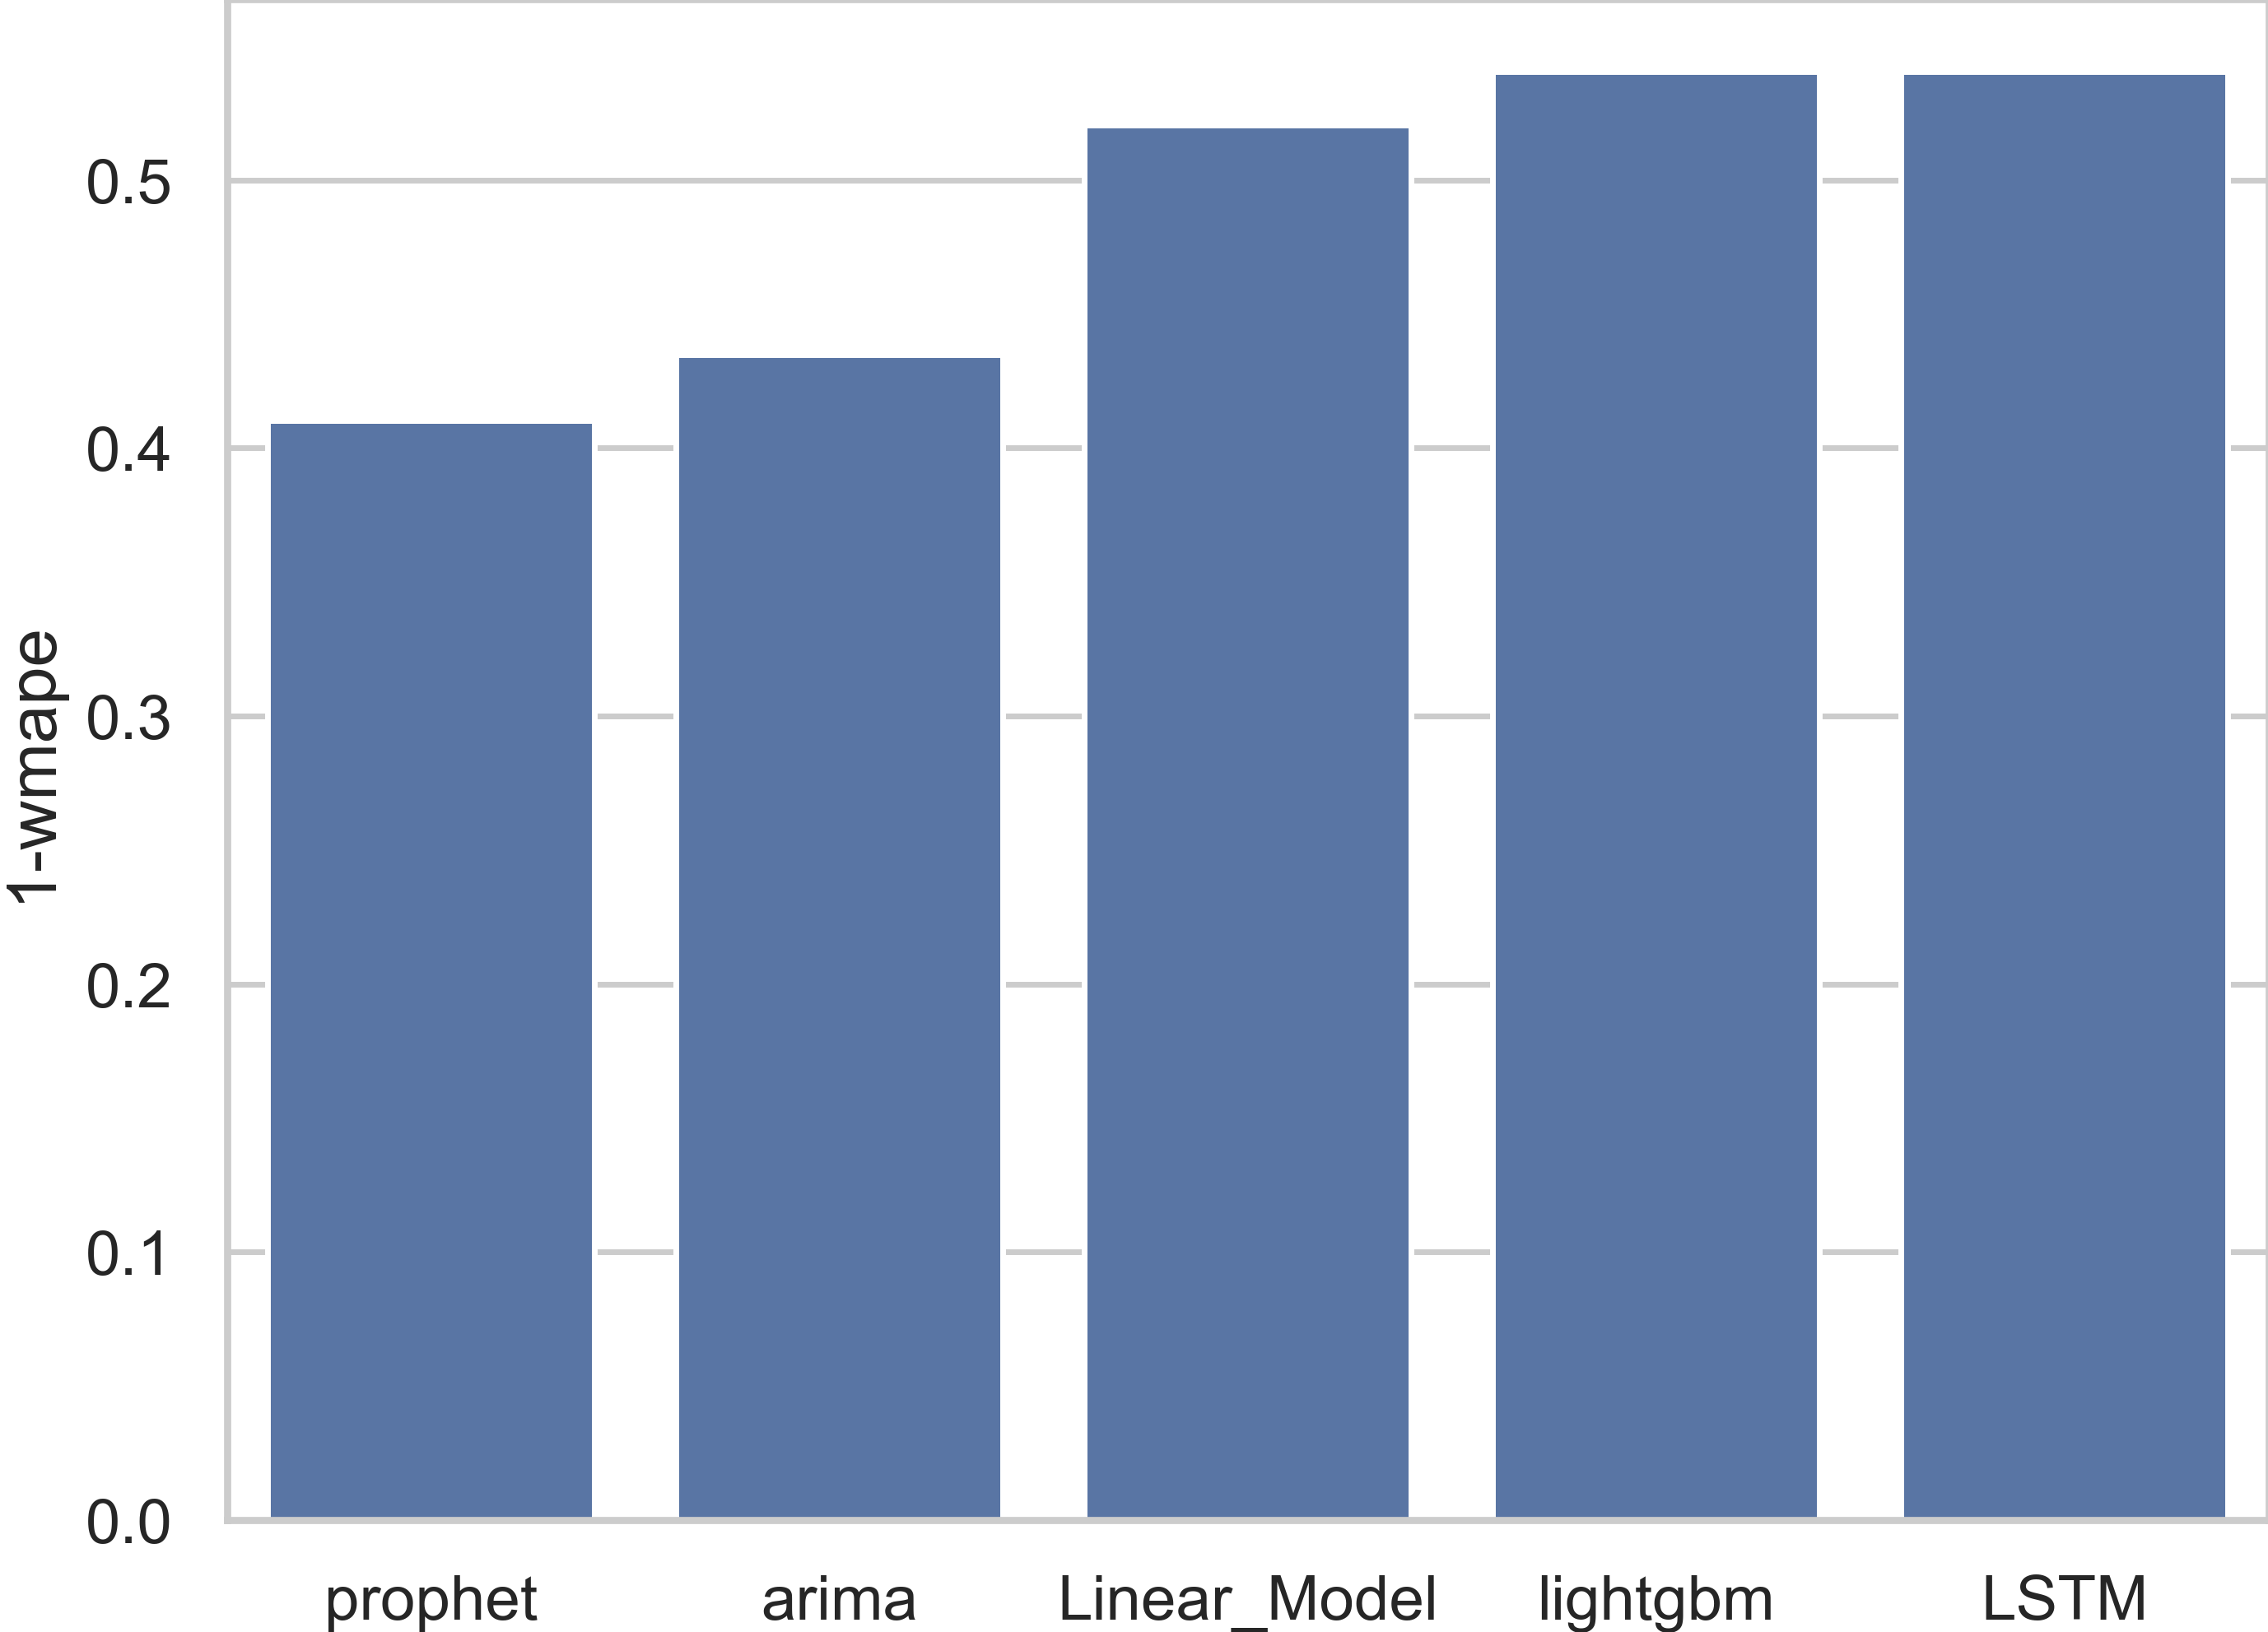
\includegraphics[width=15cm,height=9cm]{figure/模型对比.png}%figure目录存放图片
     \caption{模型对比}
     \label{模型对比}
    \end{figure}
    
  \subsubsection*{(3) 基于贝叶斯优化器的超参数优化}

  对于LightGBM算法存在许多超参数,合理的超参数可以提升模型准确度,降低模型过拟合的风险。具体的超参数包括:
  
     1)决策树剪枝超参数num\_leaves,max\_depth,
min\_child\_samples,main\_gain\_to\_split等。num\_leaves为一颗树上的叶子节点数,max\_depth为树的最大深度,min\_child\_samples为单个叶子节点上的最小样本数量,main\_gain\_to\_split为再分裂所需的最小增益。

    2)Boosting过程控制超参数:reg\_alph,reg\_lambda,n\_estimators等。reg\_alph为L1正则化系数,reg\_lambda为L2正则化系数,n\_estimators为迭代次数.
   
    3)特征和数据处理类超参数:subsample,subsample\_freq等。subsample为模型训练时抽取的样本数量,取值范围是$(0,1]$,subsample\_freq为抽样频率,表示每隔几轮进行一次抽样。
    \subsubsection*{$\bullet$ 贝叶斯优化器}

    贝叶斯优化 (Bayesian Optimization)是基于模型的超参数优化,已应用于机器学习超参数调整,结果表明该方法可以在测试集上实现更好的性能,同时相较于网格搜索,随机网格搜索,对半网格搜索等传统超参数优化器,以及基于粒子群优化算法(PSO)的超参数调优,贝叶斯算法调参速度优势显著,优化效果好。
    
    1)超参数优化问题定义:
$$argmin_{x\epsilon X} f(x)$$
    其中,$x$为超参数的一组设置取值,$X$为混合设计空间(Design Space)。$f(x)$为超参数优化中,我们需要优化的目标(如最小化Loss)。

    根据贝叶斯定理:
    $$p(A|B)=\frac{p(B|A) \cdot p(A)}{p(A)}$$
    
    $\bullet \qquad p(A)$为先验概率,即代理模型;
    
    $\bullet \qquad p(B|A)$为给定代理模型,观察数据B的分布;
    
    $\bullet \qquad p(A|B)$为后验分布,即给定观察数据B之后代理模型新分布。
    
    2)贝叶斯优化框架大致如图\ref{贝叶斯原理};

    3)其中,当黑盒函数的自变量是连续值时,高斯过程回归模型(GPs)是一个非常高效的代理模型(Surrogate Model)。对于黑盒函数,我们通常假设其符合某一个GPs先验分布。高斯过程回归模型(GPs)有如下的两方面来决定:
    
    $\bullet \quad$ 均值函数$m(x)$;

    $\bullet \quad$ 协方差函数(矩阵),或者核函数$k_\theta(x,x^')$,其中\theta为核函数超参数;

    基于上面两点,我们通常假设我们观测到的函数值$y_l$通过如下的形式产生:

    $$y_l=f(x_l)+\epsilon_l ,\epsilon_l \sim N  (0,\sigma_{noise}^2)$$

    其中$x_l$为数据集,$\epsilon_l$为误差。由此,可以得到高斯似然函数形式:

    $$y_l|x_l \sim N(f_l,\sigma_{noise}^2) $$

    其中$f_l=f(x_l),f(x)$服从如下分布:
    
    $$f(x) \sim GP(m(x),k_{\theta}(x,x^{'}))$$
    
    4)模型通过采集函数(Acquisition Function,即AC函数),来决定输出下一个采集点。

    给定先验和观察数据,由贝叶斯定理得到相应的后验分布:
    
    后验分布=先验分布+观察数据

    AC函数时根据后验分布$p_\theta (f(\cdot)|D)$来构造的。再选定$GP_s$作为代理模型的条件下,其后验分布仍然是高斯分布:

    $$p(f(x_{1:q}|D)=N(\mu_{\theta}(x{1:q}),\sum_{\theta}(x_{1:q}))$$

    我们采用了上置信边界UCB(Upper condence bound)),作为AC函数:

$$UCB(x)=\mu(x)+\beta_t^{\frac{1}{2}} \sigma(x)$$

    第一项为均值,注重于开发,第二项为方差注重探索,β越大,说明越注重探索。

$\bullet$优化结果
    
   为了找出适用于数据集的LightGBM的具体参数,我们将LightGBM预测的1-wmape作为优化的目标函数,通过不断地添加样本点来更新目标函数的后验分布,从而更好的调整当前的参数。
  
    \begin{figure}[htbp]
     \centering
     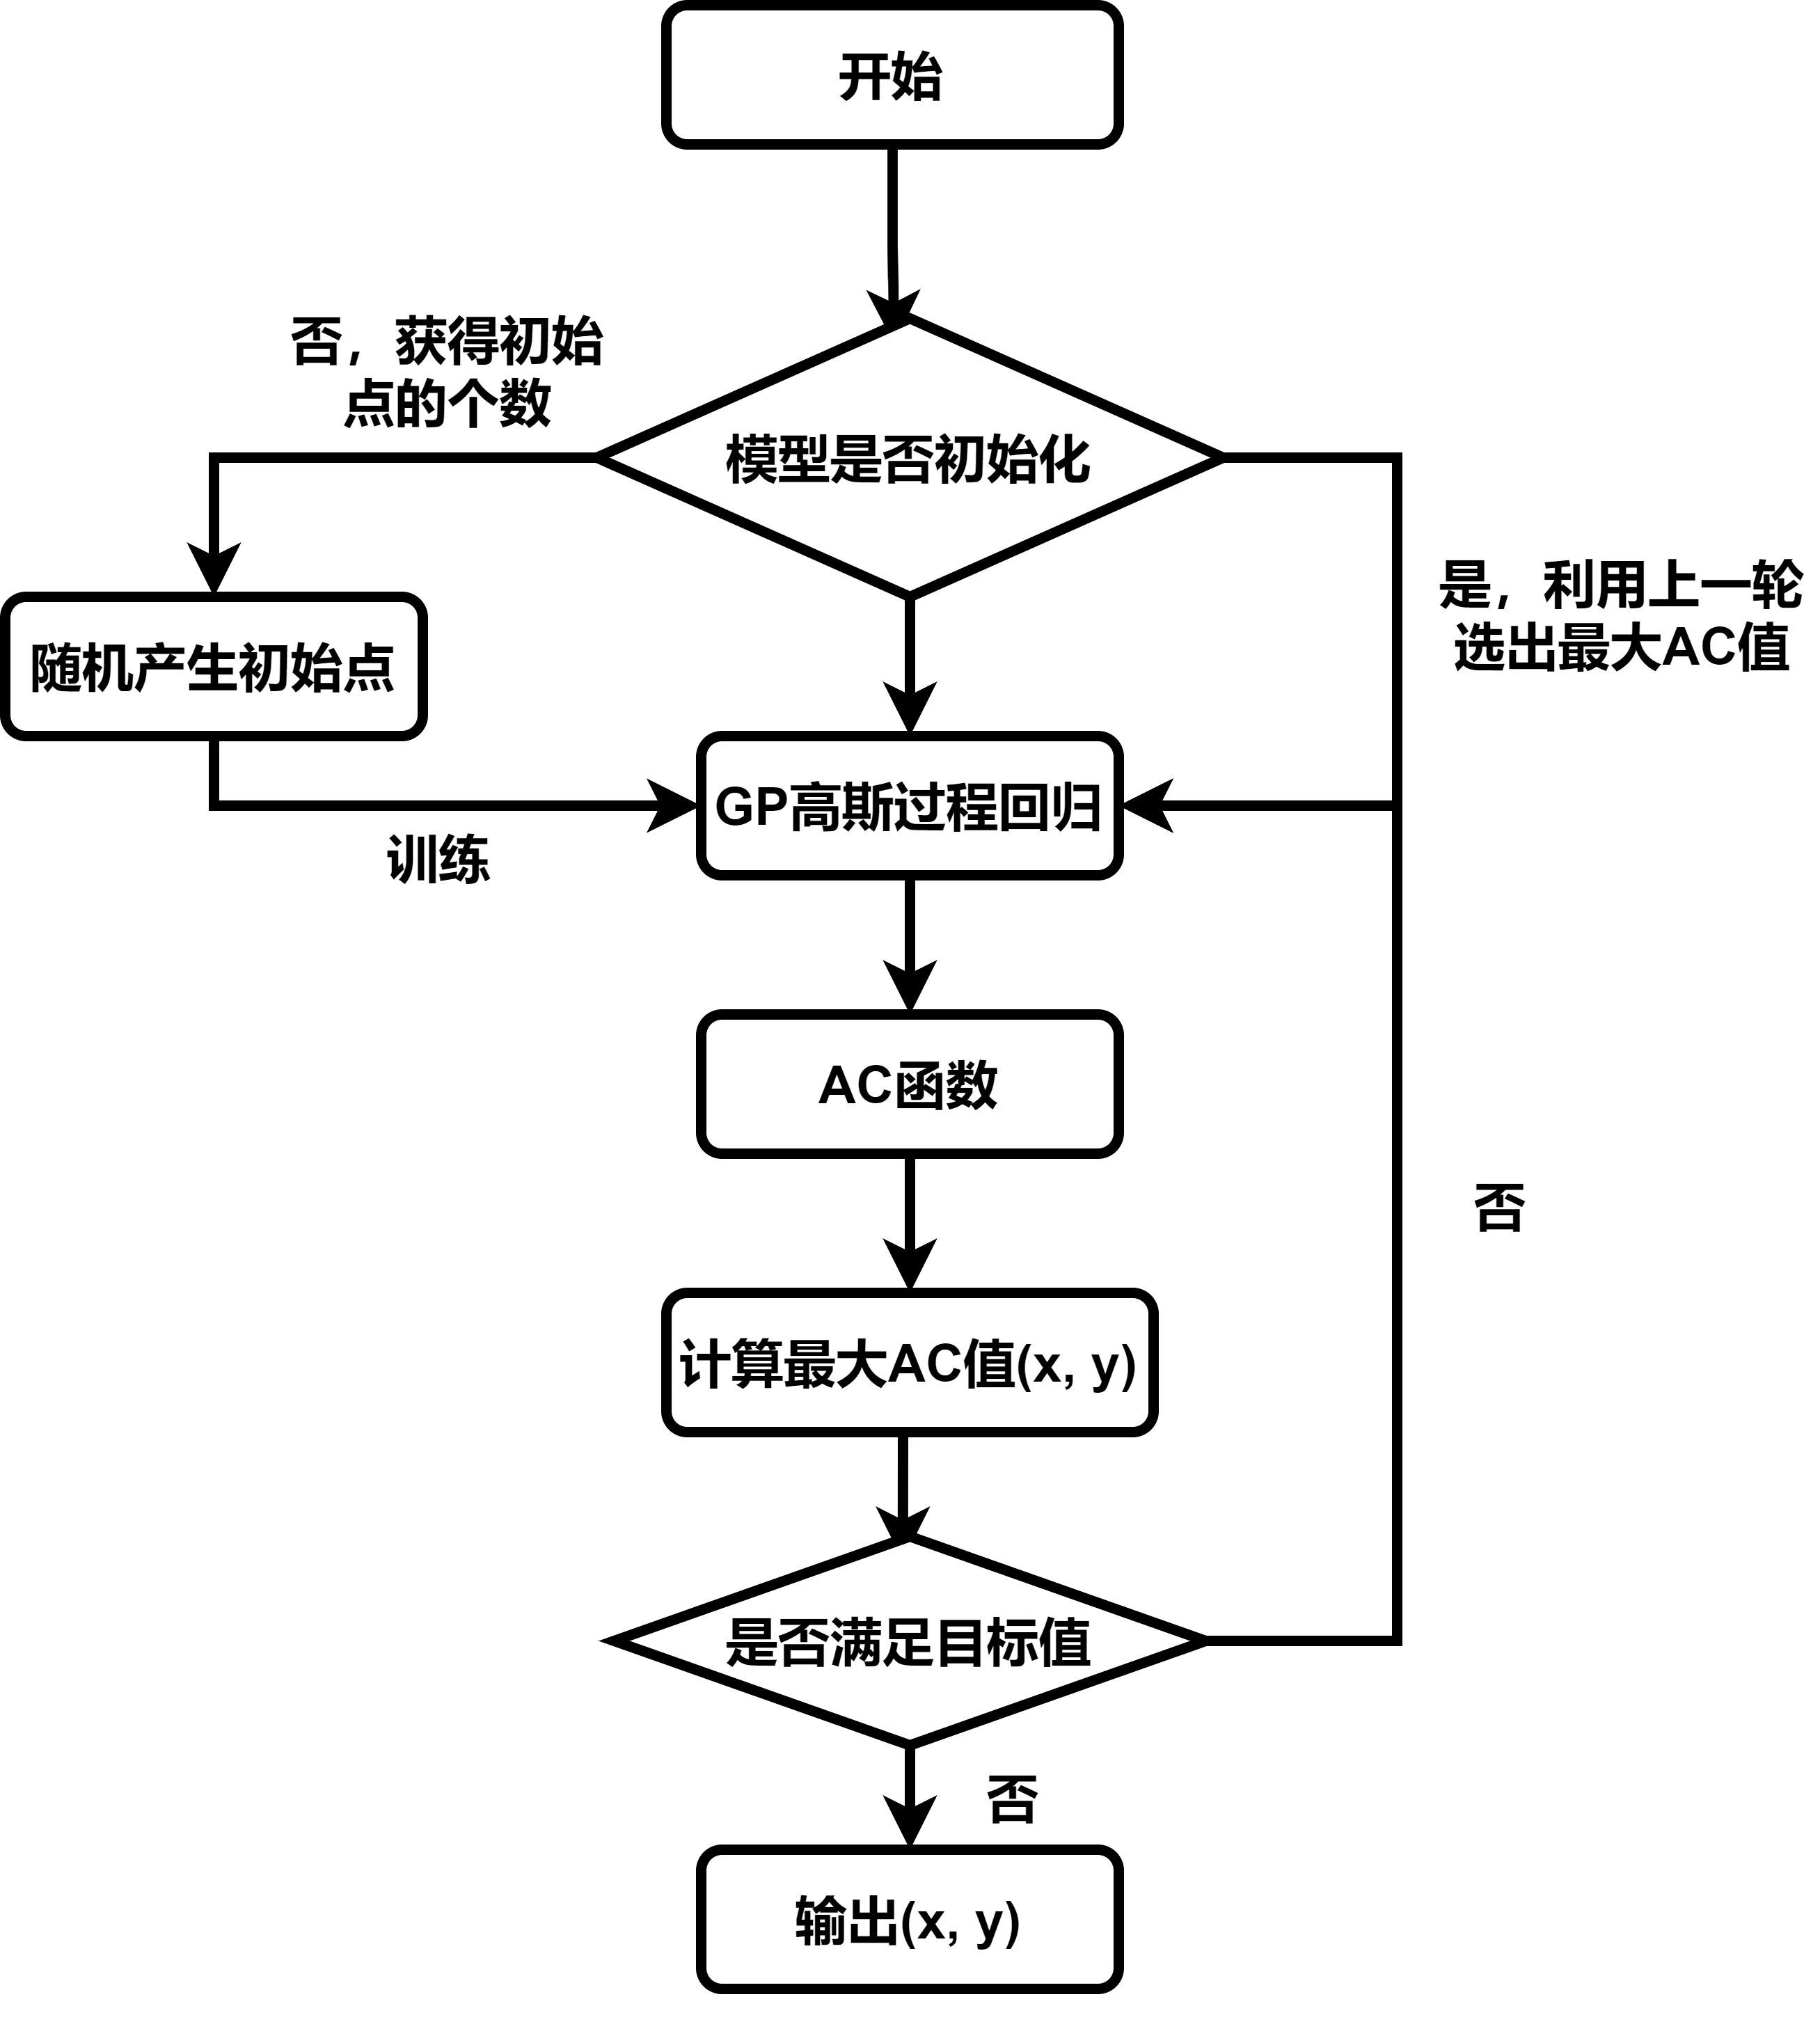
\includegraphics[width=14cm,height=15cm]{figure/贝叶斯.png}%figure目录存放图片
     \caption{贝叶斯原理}
     \label{贝叶斯原理}
    \end{figure}

    贝叶斯优化器执行不同次数时,以1-wmape为指标的模型准确度如图\ref{贝叶斯调参}所示,我们可以看到当贝叶斯优化器执行24次时,1-wmape为0.534为LightGBM效果最好的时候,此时具体超参数可以见表1。

  

    \begin{figure}[htbp]
     \centering
     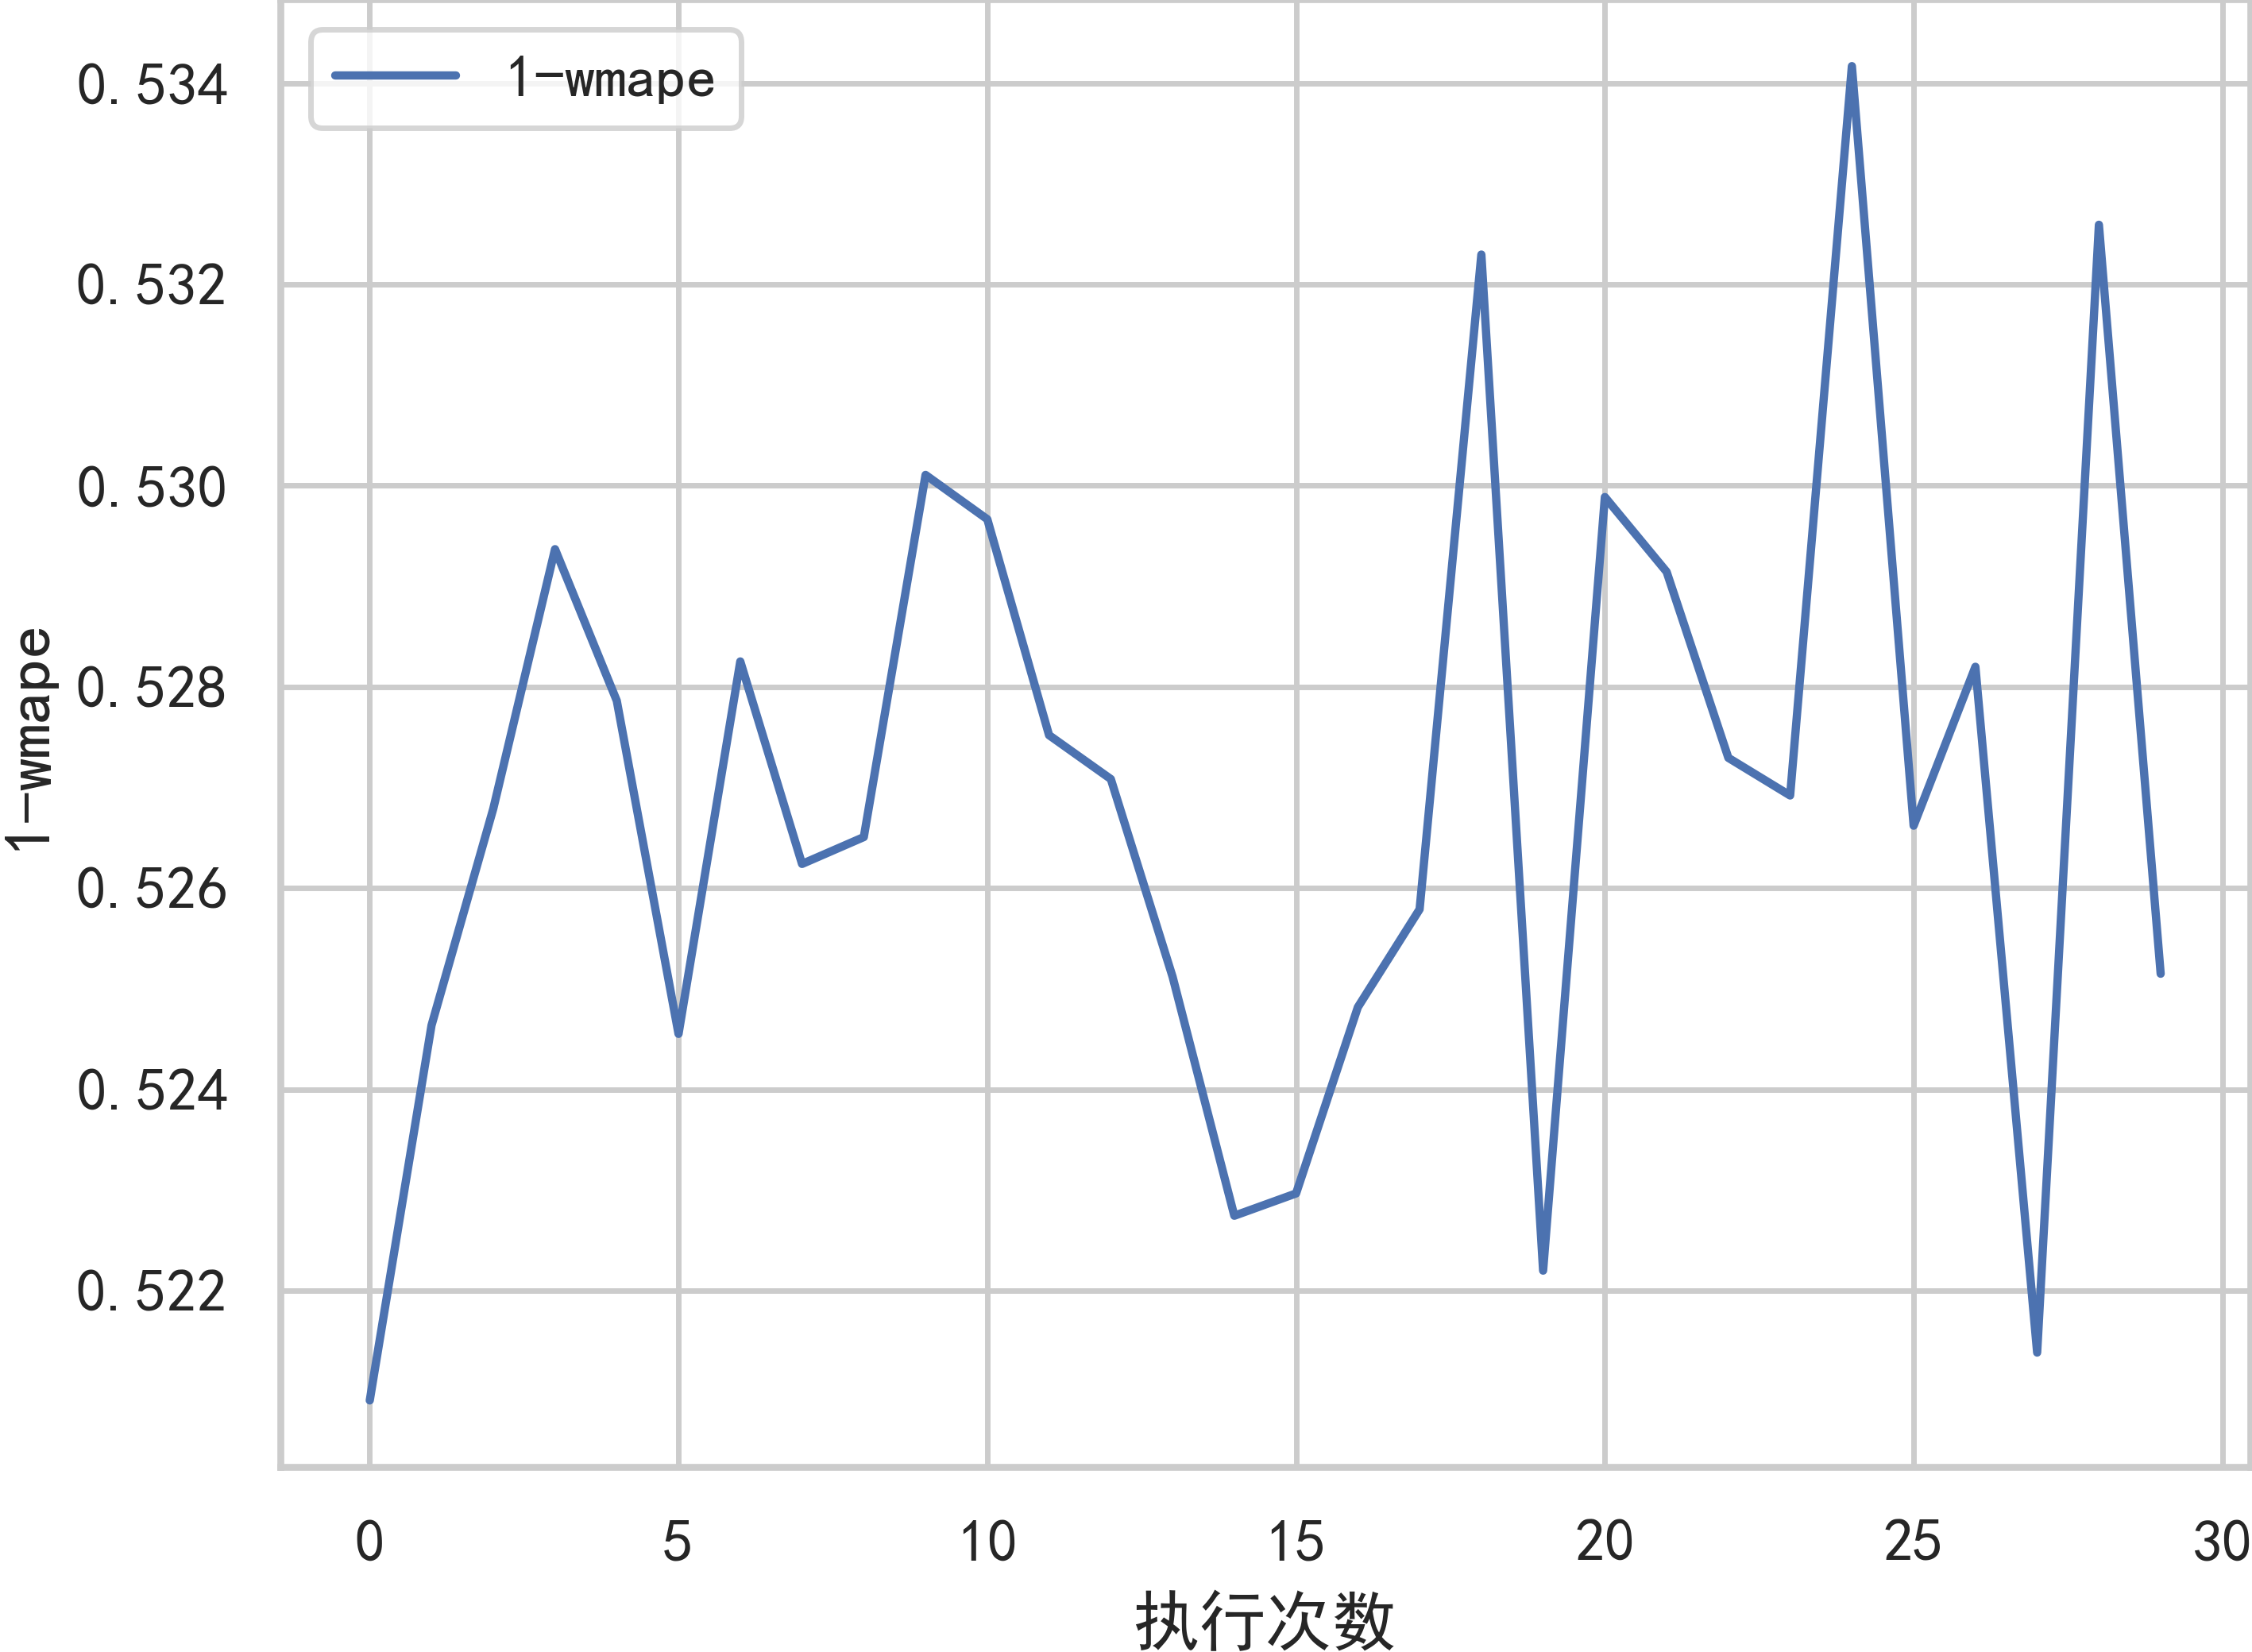
\includegraphics[width=15cm,height=10cm]{figure/贝叶斯调参.png}%figure目录存放图片
     \caption{贝叶斯调参}
     \label{贝叶斯调参}
    \end{figure}

\begin{table}[htbp]
  \centering
  \label{优化结果}
  \caption{优化结果}
  \begin{tabular}{ccccc}
   \toprule
    ~~~~ & 超参数 & ~~~~~~~~~ & 优化结果 & ~~~~ \\
   \midrule
   ~~~~ & max\_depth & ~~~~~~~~~ & 8 & ~~~~ \\
   ~~~~ & min\_child\_samples & ~~~~~~~~~ &  154 & ~~~~ \\
   ~~~~ & min\_gain\_to\_split & ~~~~~~~~~ & 0.6833583331773246 & ~~~~ \\
   ~~~~ & n\_estimators & ~~~~~~~~~ & 55 & ~~~~ \\
   ~~~~ & num\_leaves & ~~~~~~~~~ & 592 & ~~~~ \\
   ~~~~ & reg\_alph & ~~~~~~~~~ & 7.272509971489392 & ~~~~ \\
   ~~~~ & reg\_lambda & ~~~~~~~~~ & 8.903467966901635 & ~~~~ \\
   ~~~~ & subsample & ~~~~~~~~~ & 0.963070322738298 & ~~~~ \\
   \bottomrule
\end{tabular}
\end{table}
    
\subsubsection{结果的分析}
 最终我们预测出结果,其中一条时间序列结果如下图\ref{时间序列结果},我们预测模型的1-wmape结果为0.534,具体结果见附件结果。
  \begin{figure}[htbp]
     \centering
     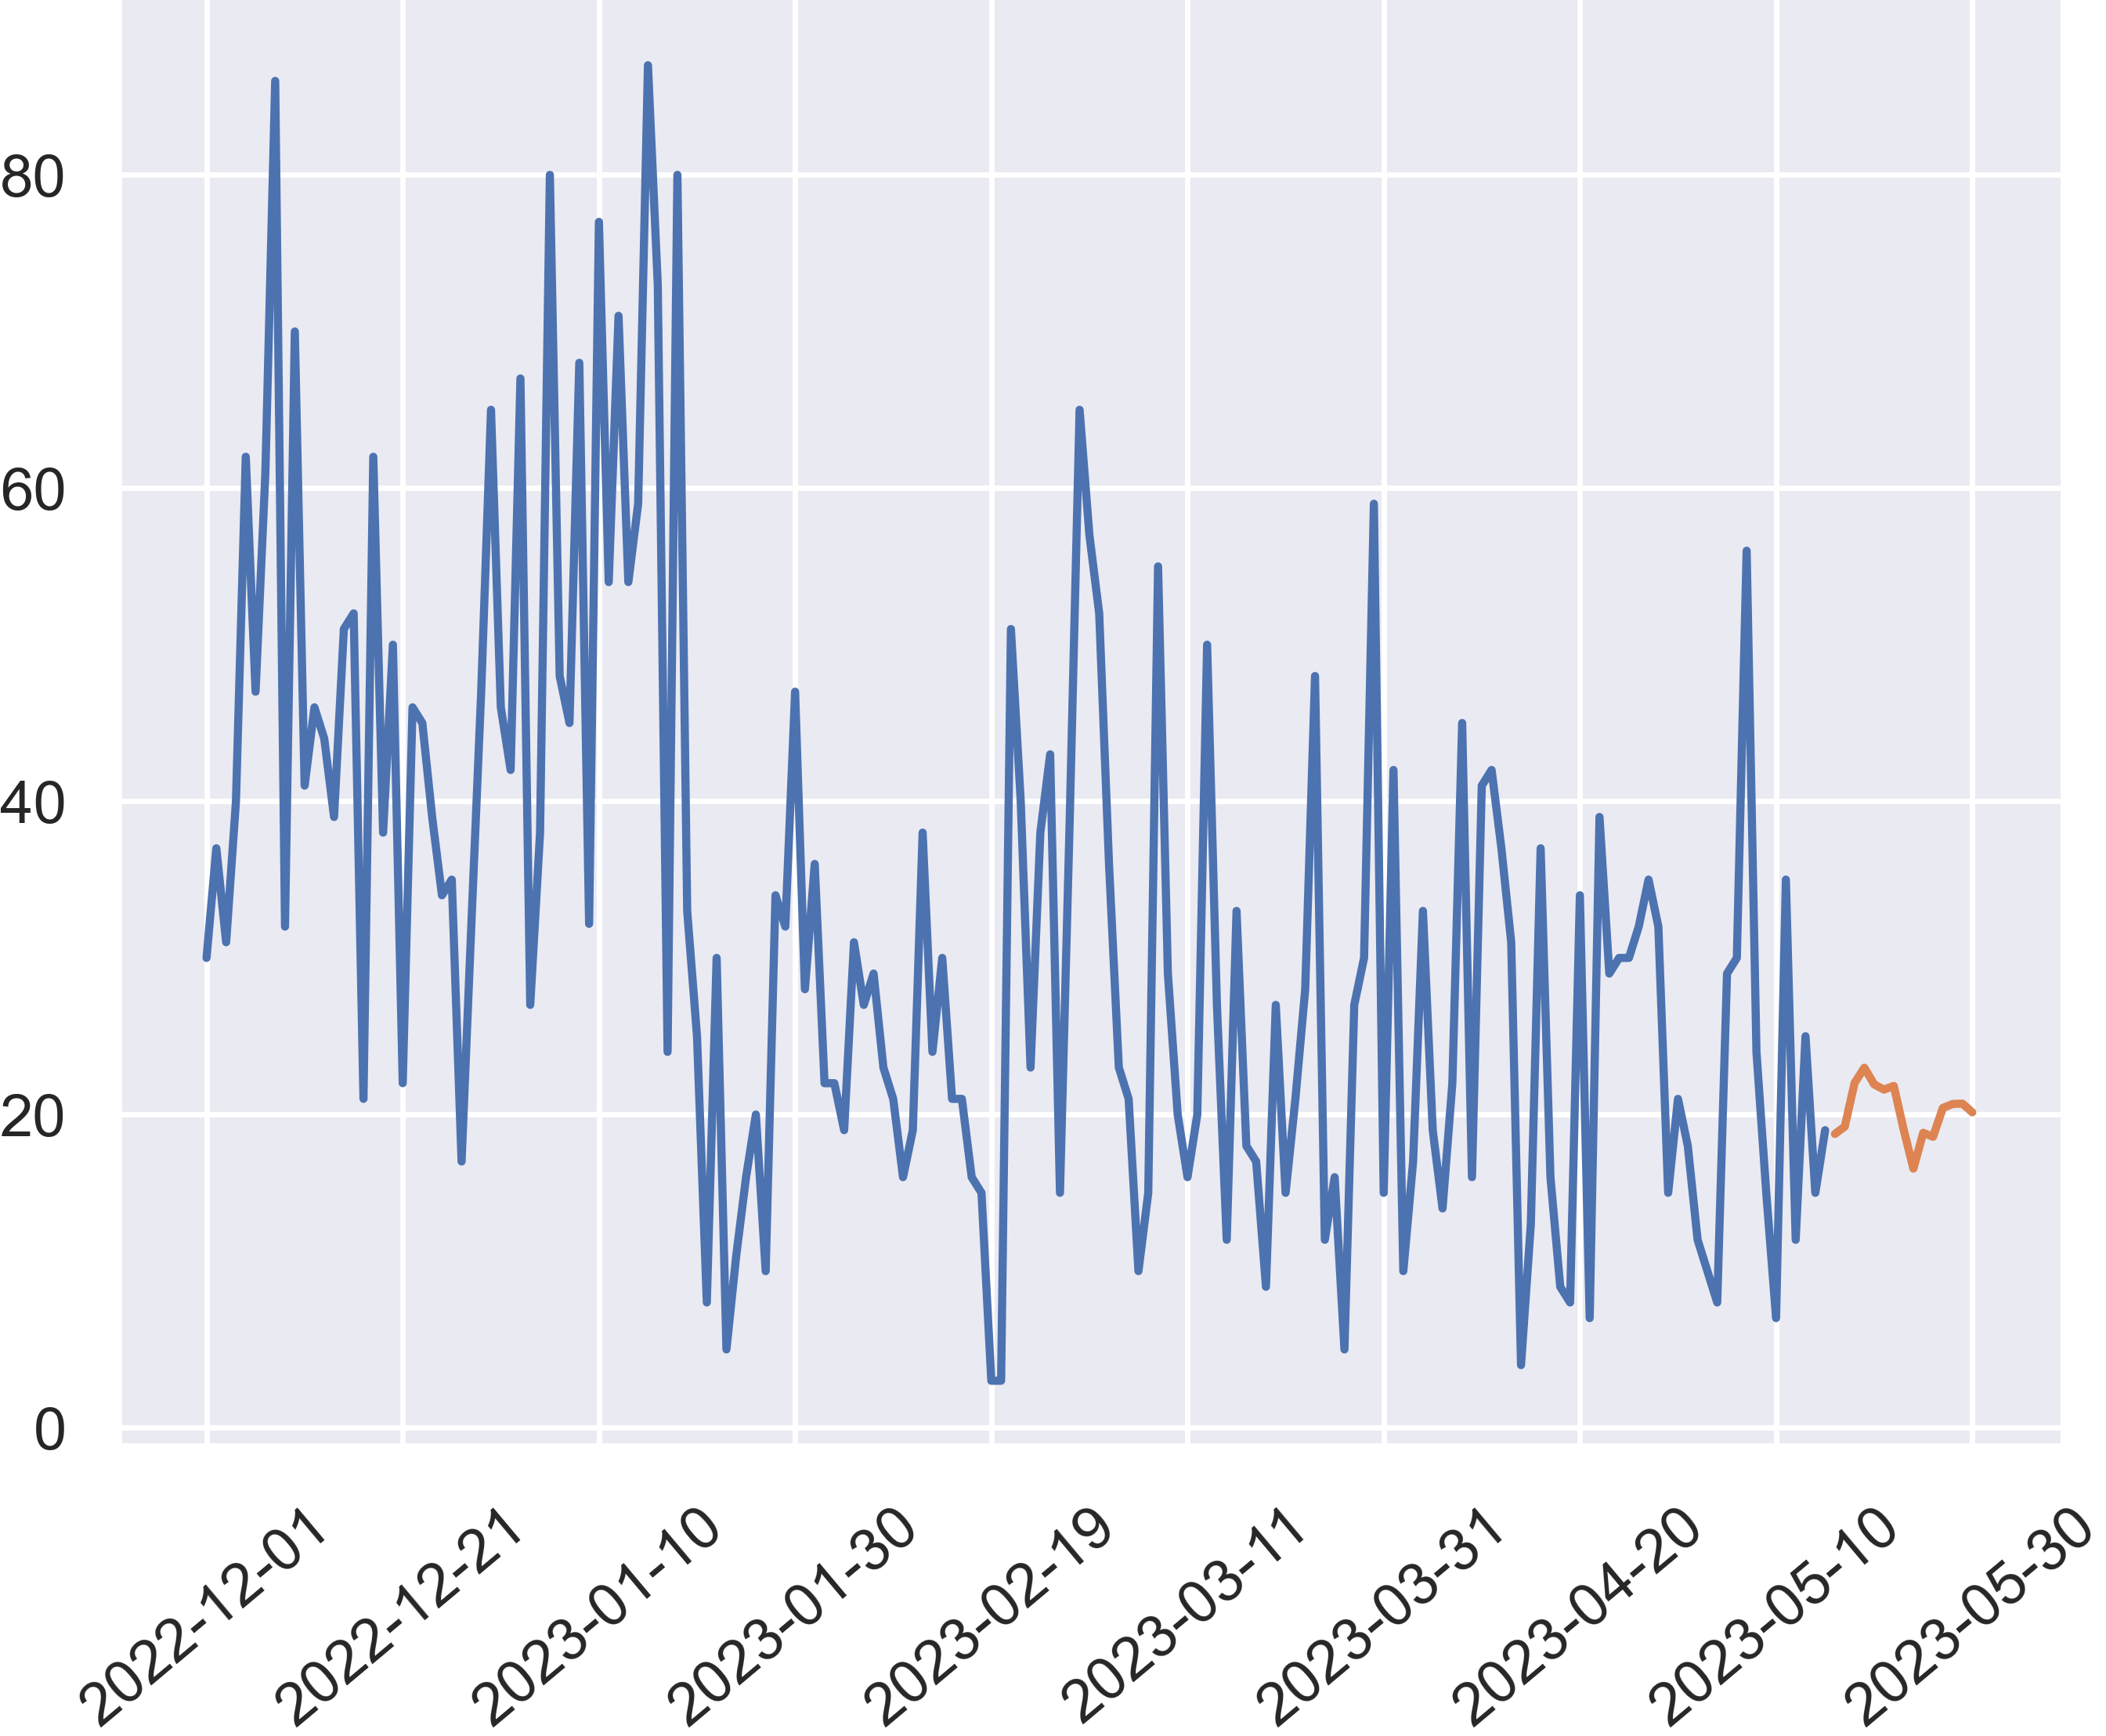
\includegraphics[width=15cm,height=10cm]{figure/第一条时间序列结果.png}%figure目录存放图片
     \caption{时间序列结果}
     \label{时间序列结果}
    \end{figure}
\subsection{问题二的建模和求解}
\subsubsection{模型的建立}
对于问题二,我们采用问题一中建立的模型来进行预测和分析。具体而言,我们使用附件5的数据进行如第一问的数据处理,然后将这些数据集输入问题一模型中,模型将根据这些数据进行预测。最后,我们根据模型的预测结果来分析问题二中的数据,并得出相应的结论。

通过对附件5中新出现的商家和新产品的维度进行部分可视化分析,我们可以明显看出该条件下数据集的分布与以前有部分相似之处。在问题一的模型中,我们的团队针对四个附件的所有特征进行了独热编码,尽可能考虑到所有特征之间的关联性,因此第一问的模型依旧适用于第二问。
    \begin{figure}[htbp]
      \centering
        \begin{subfigure}{0.4\textwidth}
          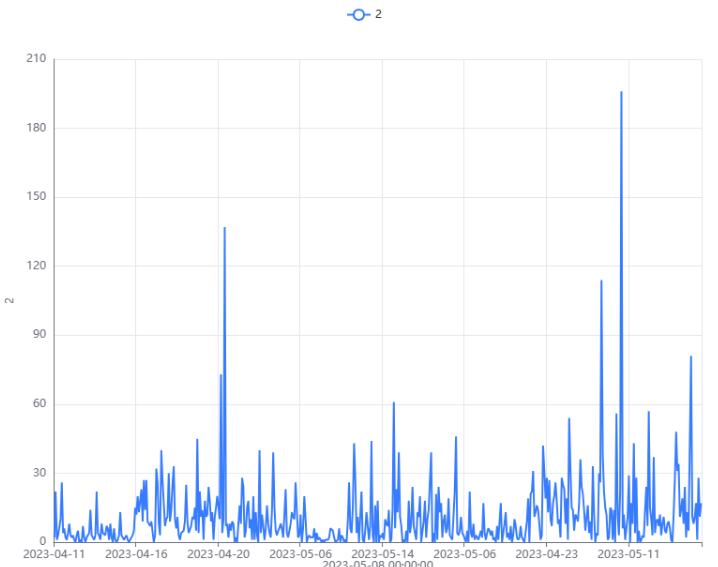
\includegraphics[width=\textwidth]{figure/附件5某商家的时间序列.png}
          \caption{附件5某商家的时间序列}
          \label{附件5某商家的时间序列}
        \end{subfigure}
        \begin{subfigure}{0.4\textwidth}
          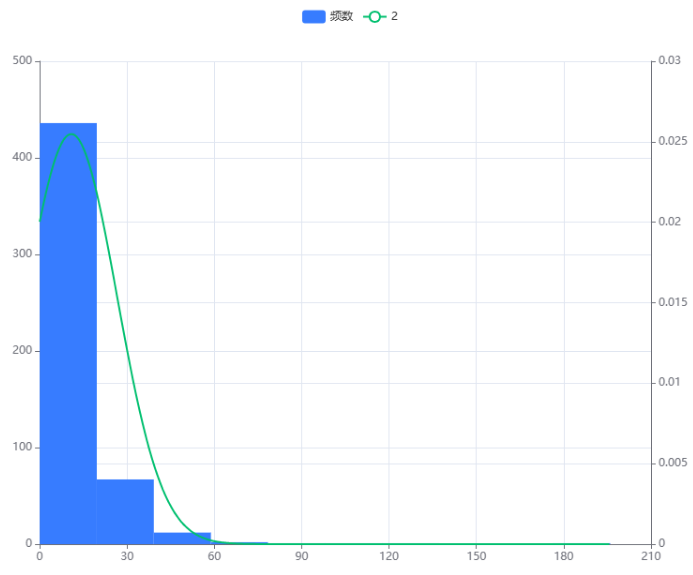
\includegraphics[width=\textwidth]{figure/附件5某商家的正态分布.png}
          \caption{附件5某商家的正态分布}
          \label{附件5某商家的正态分布}
        \end{subfigure}
    \end{figure}
\subsubsection{模型的求解}
  通过使用问题一的模型,我们得到最终结果。
\subsubsection{结果的分析}
  最终我们预测出结果,其中一条时间序列结果如下图\ref{第二问时间序列结果},由图可见原先数据集具有明显的按月的周期性规律,并在某一时间点达到最大值。预测的结果基本上具有此类变化和规律,说明预测比较合理,具体结果见附件结果。
  \begin{figure}[htbp]
     \centering
     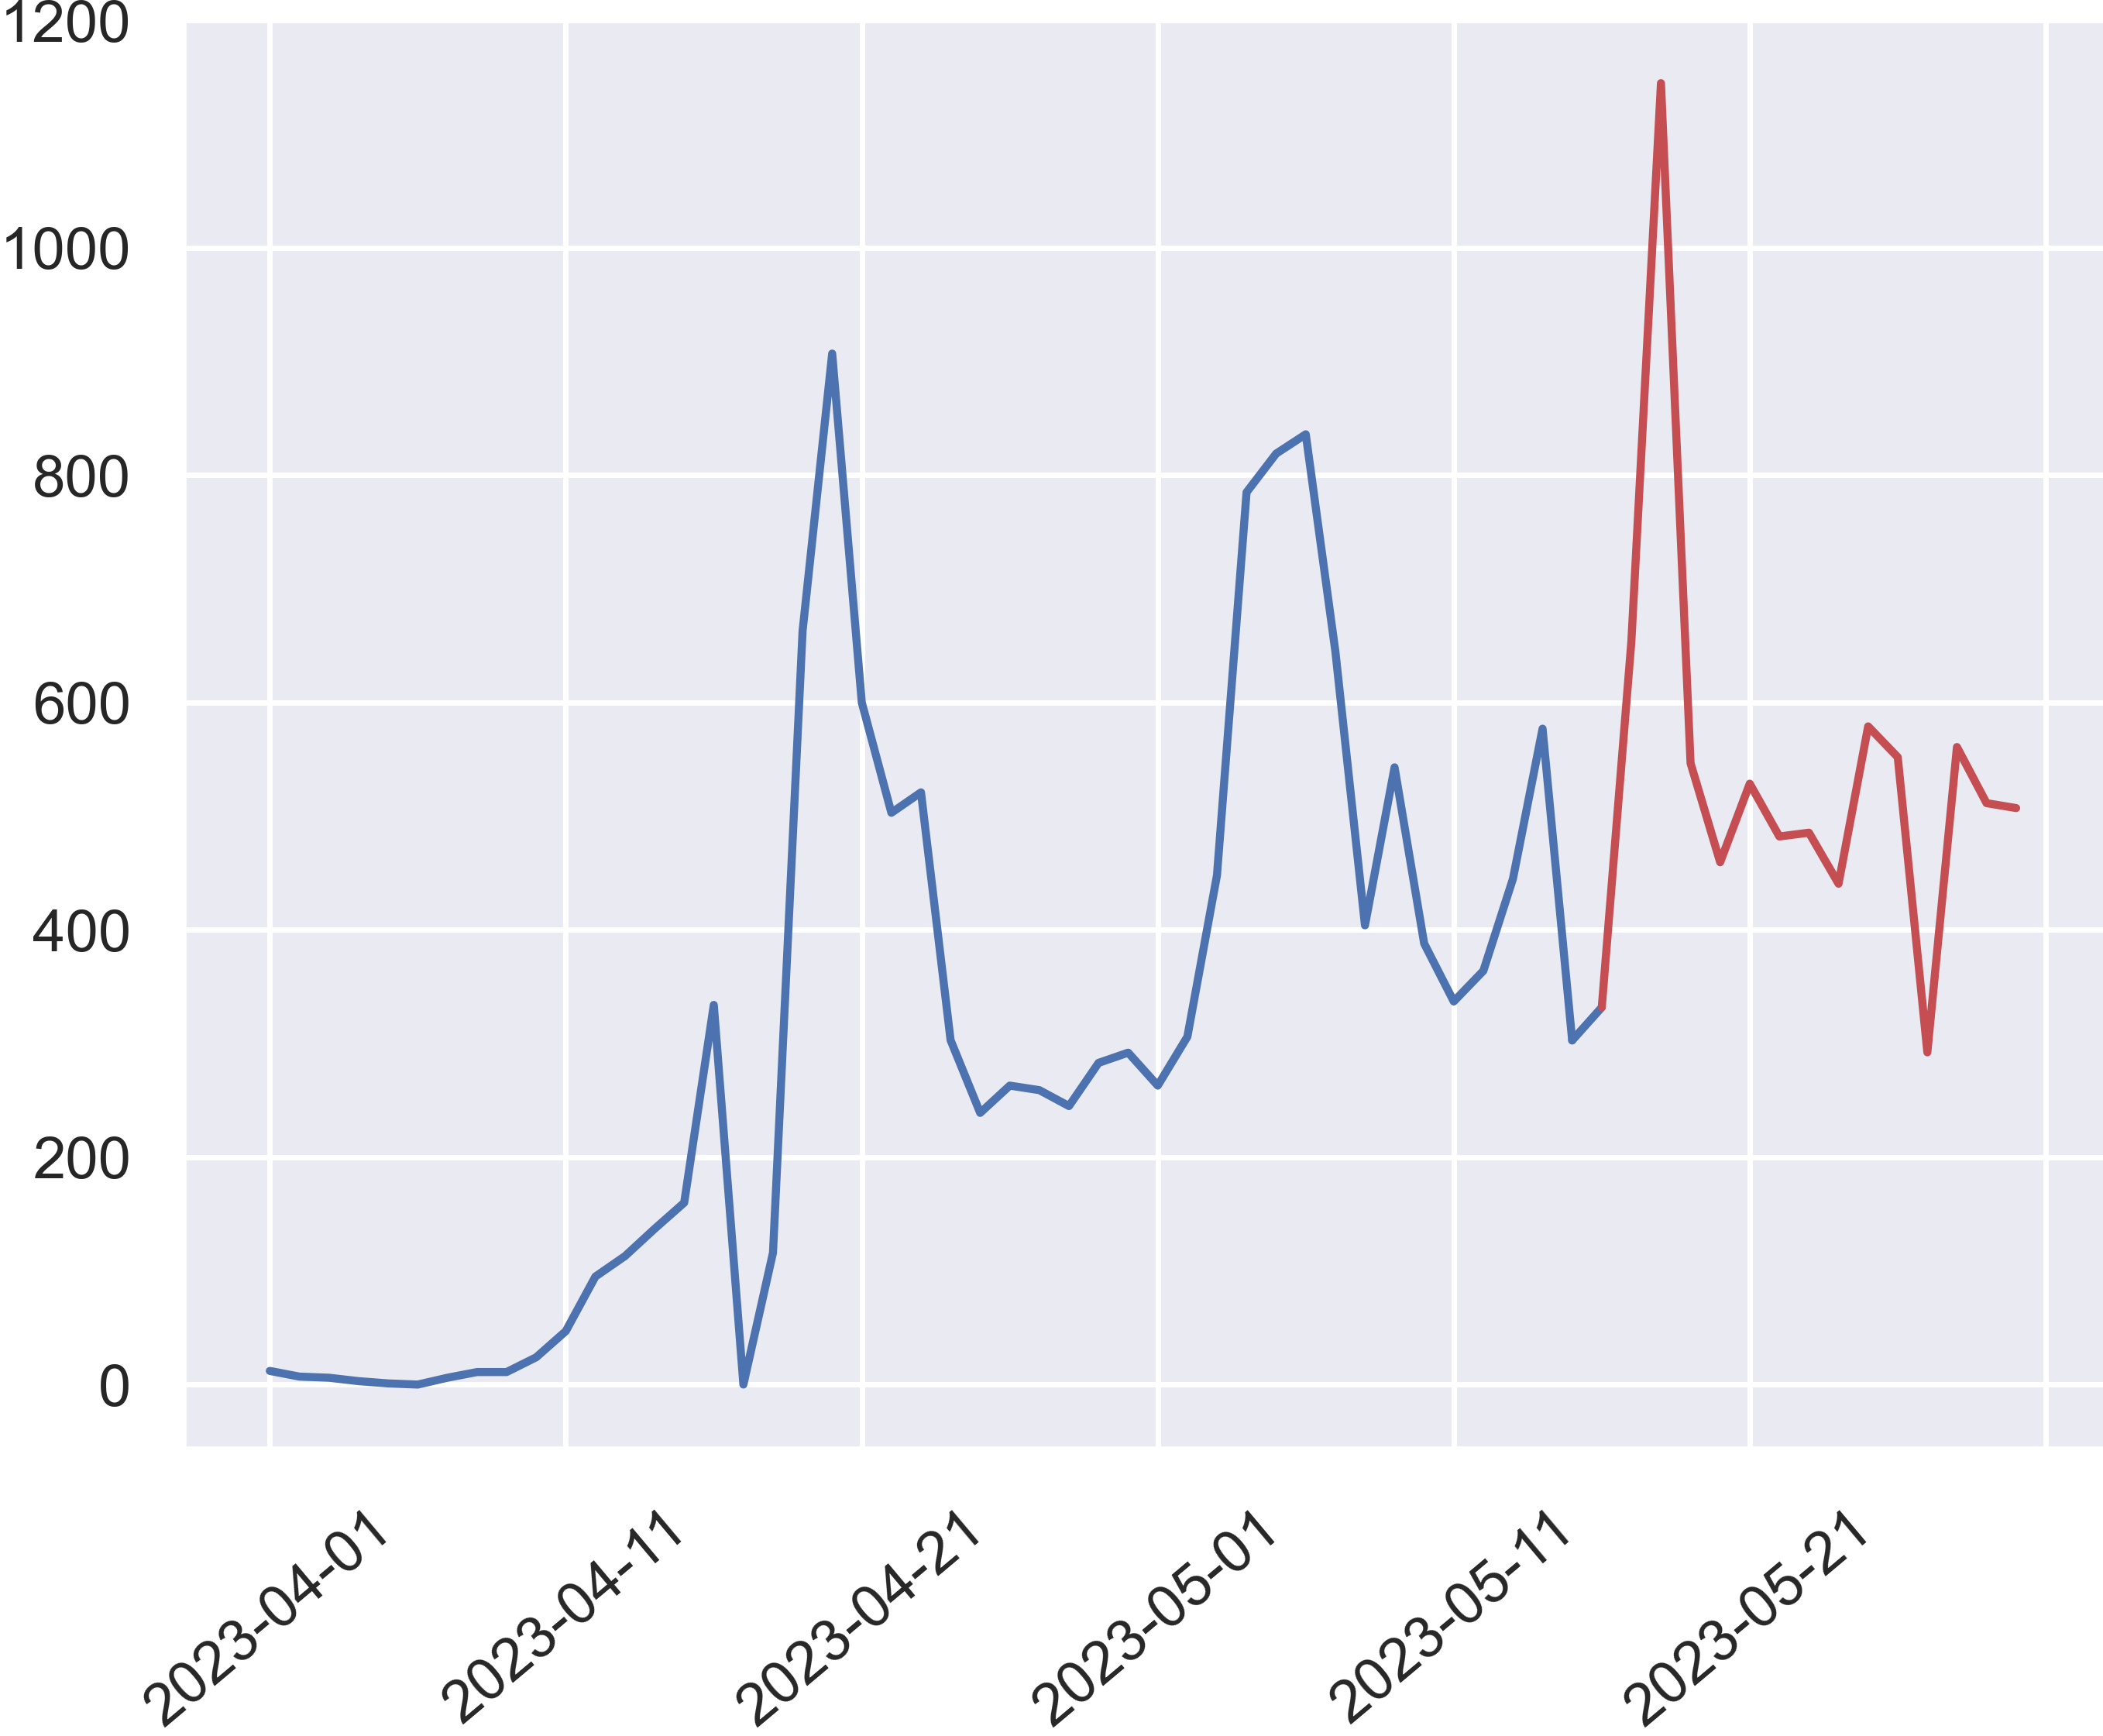
\includegraphics[width=15cm,height=10cm]{figure/第二问时间序列结果.png}%figure目录存放图片
     \caption{时间序列结果}
     \label{第二问时间序列结果}
    \end{figure}

\subsection{问题三的建模和求解}
\subsubsection{模型的建立}
  对于第三问,我们应该考虑现规律性的大型促销对预测结果的影响,通过引入变量promote来描述是否该时间段是否处于促销时期。
当不处于促销时期时promote设为0,当处于促销时期设为1,再使用LightGBM算法对6月促销期的时间序列进行预测。
\subsubsection{模型的求解}
  首先,我们使用附件6中的数据,并进行预处理,然后,我们对时间序列进行聚类,然后判断该时间段是否处于促销时期,以此来引入promote变量,然后使用LightGBM算法根据这些数据进行预测。
\subsubsection{结果的分析}
  最终我们预测出结果,其中一条时间序列结果如下图\ref{第三问时间序列结果},由图可见,在6月份进入促销期,出货量不断上升,这说明我们的模型比较合理,具体结果见附件结果。
  \begin{figure}[htbp]
     \centering
     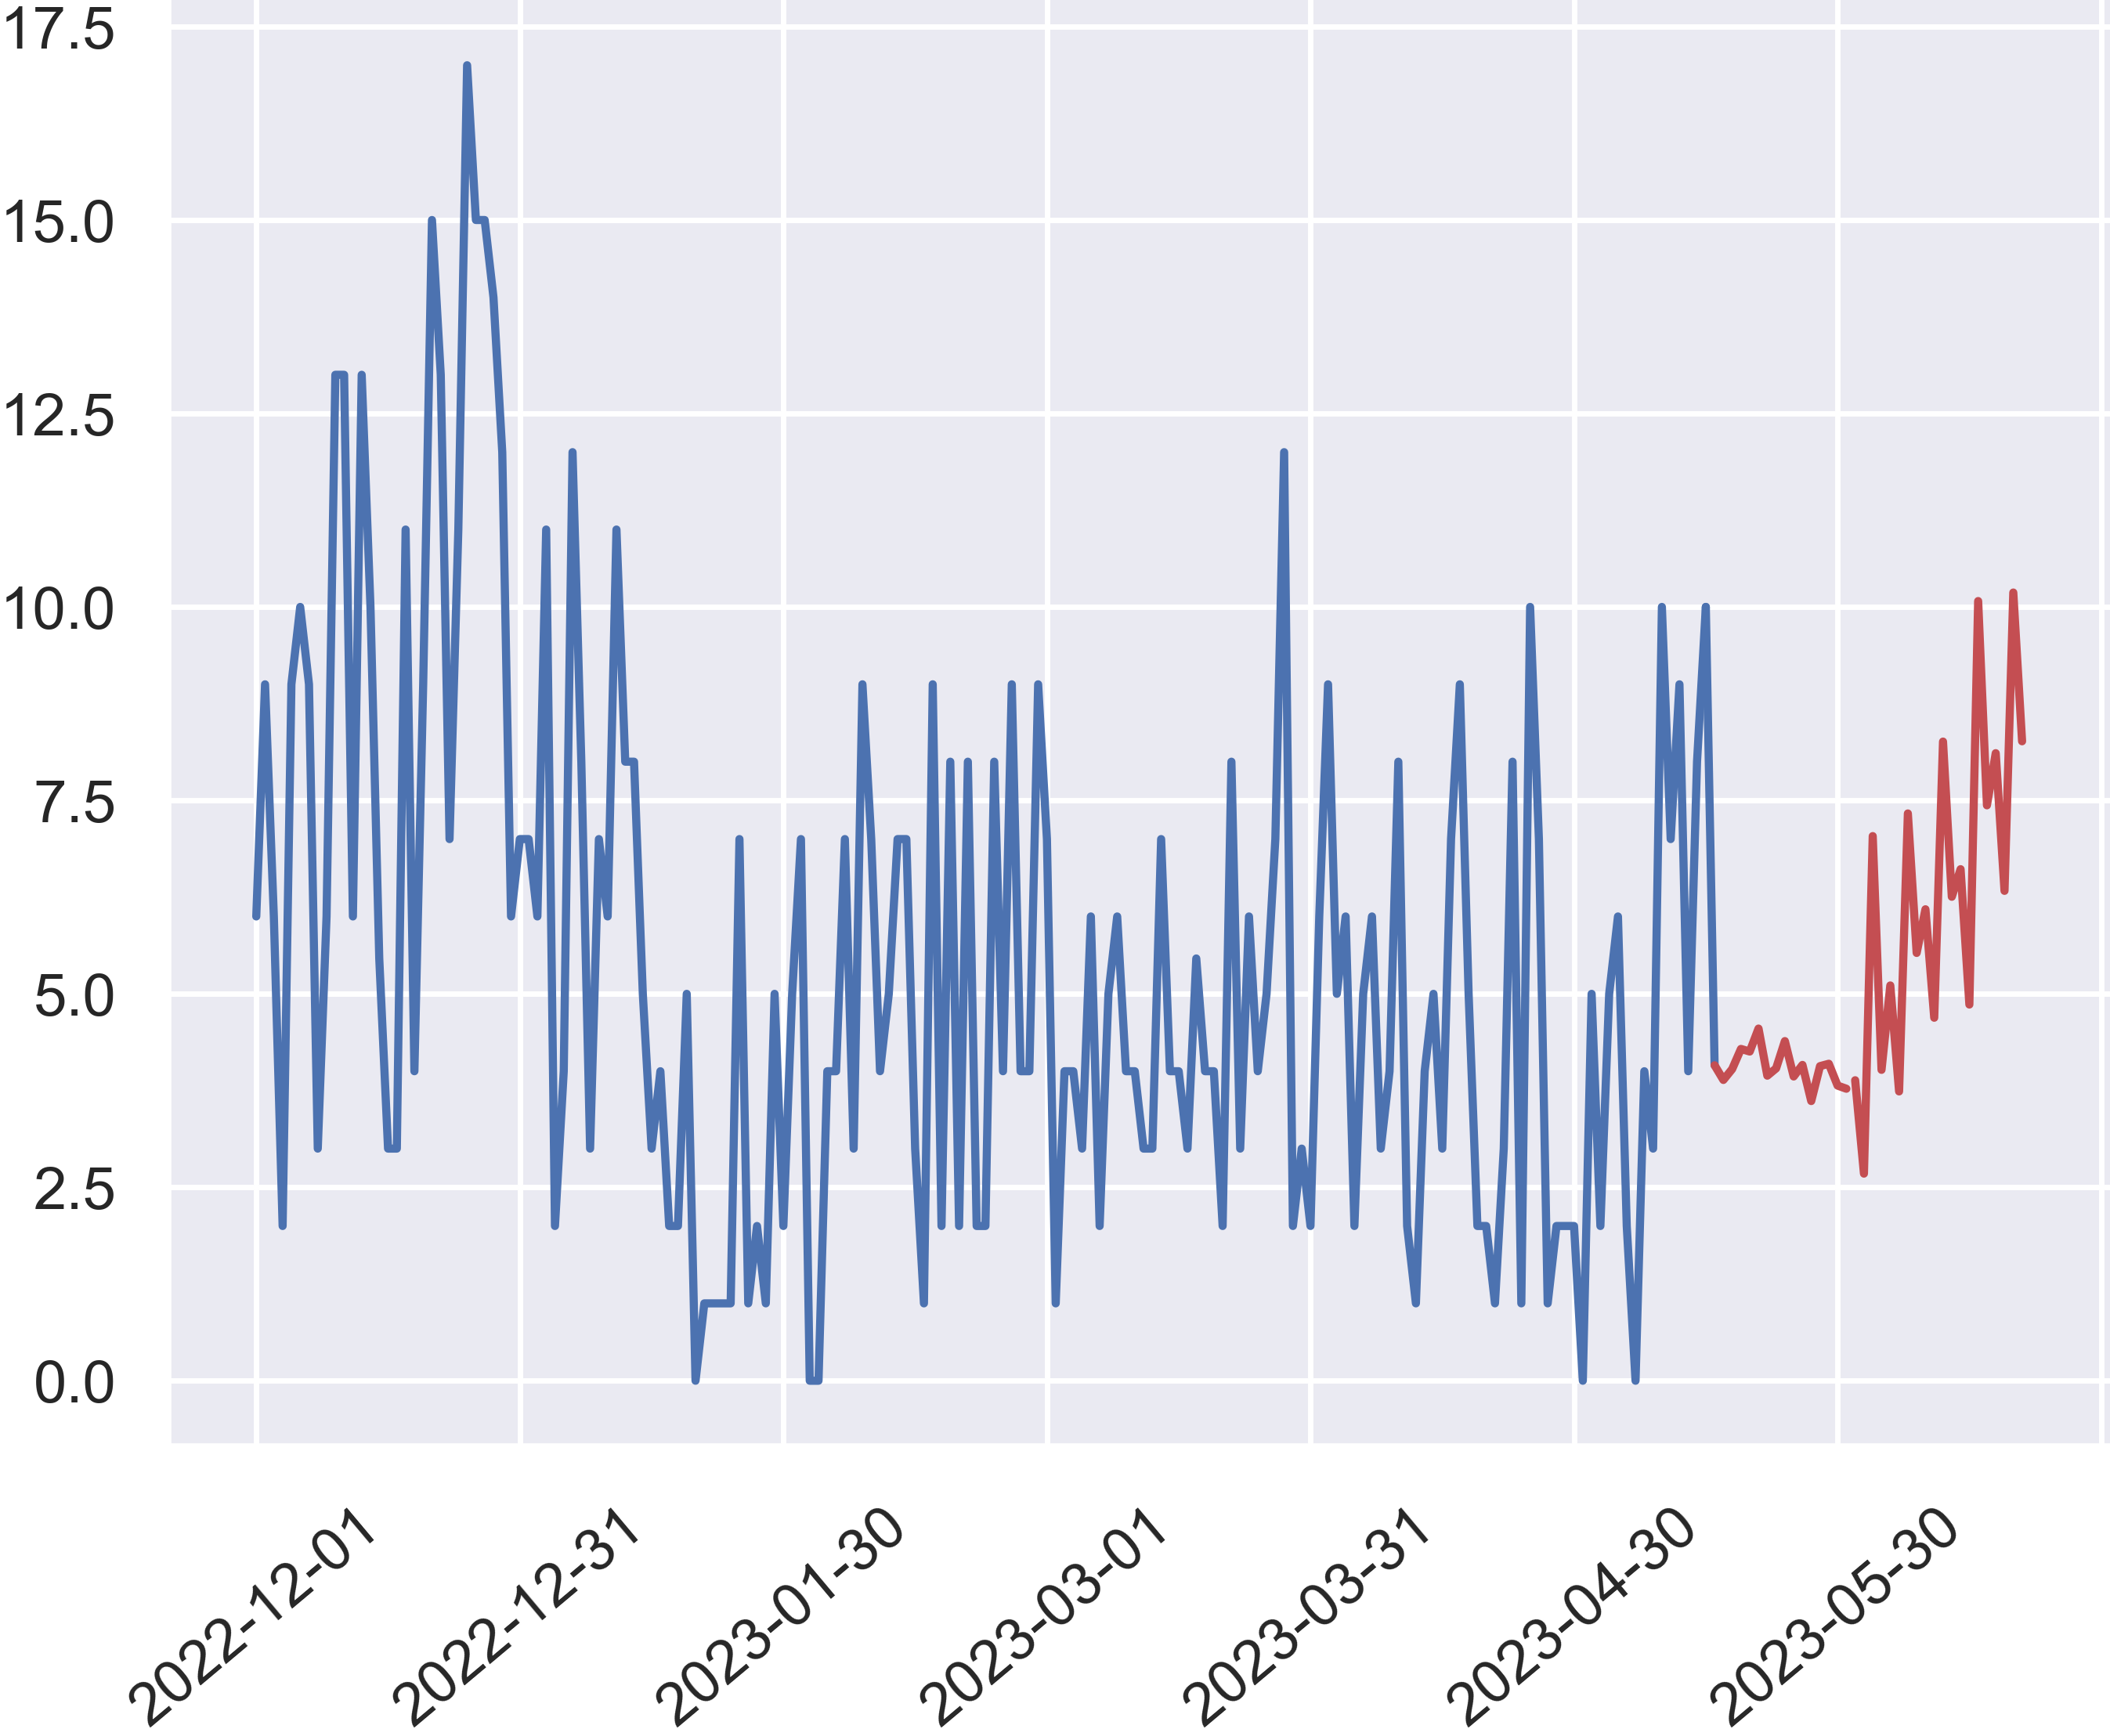
\includegraphics[width=15cm,height=10cm]{figure/第三问时间序列结果.png}%figure目录存放图片
     \caption{时间序列结果}
     \label{第三问时间序列结果}
    \end{figure}
  

\section{模型的推广和评价}
\subsection{模型的优点}
 \begin{enumerate}
\item 我们使用LightGBM模型,可以快速地训练和预测,具有低内存使用的特点,特别适合处理大规模数据,不会因为内存限制而无法处理大数据集。预测结果相较于Arima等模型更加精准。
\item 我们使用贝叶斯调参,充分考虑之前的参数信息,并不断地更新先验,迭代次数少,速度快。这种方法可以帮助我们在相对较少的评估次数内找到最优的超参数组合。贝叶斯还可以自适应地调整搜索空间,避免在低效的区域中浪费时间。
\item 我们使用时间序列聚类,通过时间序列聚类,将不同的时序数据进行划分,然后分而分析之,可以在一定程度上简化数据分析过程。相比直接预测,加入时间序列聚类后的预测方法更加准确。
\item 针对促销时间段,我们引入变量来描述该时间段是否处为促销时间,这样使我们模型对促销时间的销量的预测更加精准。
\end{enumerate}
\subsection{模型的缺点}
     \begin{figure}[htbp]
     \centering
     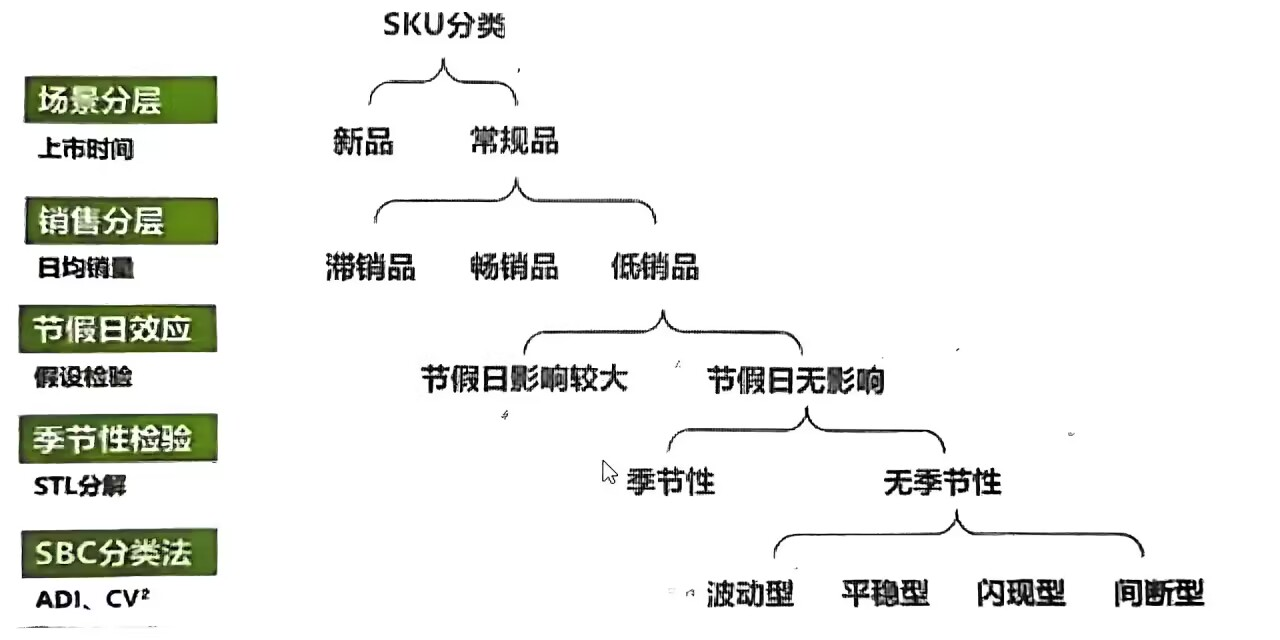
\includegraphics[width=15cm,height=8cm]{figure/更好的分类.jpg}%figure目录存放图片
     \caption{分类优化}
     \label{分类优化}
    \end{figure}
\begin{enumerate}
    \item 根据图\ref{分类优化},我们团队的分类还需要进一步优化和改进。在对时间序列进行简单分类之后,可以进行预测模型的选择及组合,不同类型的时间序列选择不同的“模型池”,再通过模型的自动筛选及组合机制将模型池里的算法模型预测结果进行组合。这会让预测结果更加准确。
	\item 预测结果有很大的提升空间,相较于融合模型,LightGBM预测结果较低。但相比部分单一模型,我们团队选取的算法模型迭代速度更快,极大缩短了时间。
    \item 我们采用了时间序列滚动窗口的方法,随着预测时间的推移,我们观察到预测误差逐渐增大的趋势。随着时间的推移,模型的预测准确性逐渐降低,导致误差逐渐积累。对于时间滚动窗口大小的选择还需要进一步调整,让其更加符合实际销售。
\end{enumerate}
\subsection{模型的推广}
\begin{enumerate}
	\item 可以使用Stacking等模型来预测时间序列,提升预测精度。
    \item 可以增加时间序列聚类的指标数,从而是一类的时间序列更加相似
    \item 可以调整时间序列滚动窗口的大小,从而提高模型预测的精度。
\end{enumerate}
  


\newpage
\begin{thebibliography}{99}
   \bibitem{a}姜向荣. \emph{季节性预测建模及其在短期宏观经济预测中的应用}[J].  统计与决策, 2019, 35(16): 75-78.
   \bibitem{b}段然,庞建华,张良钧. \emph{基于 SARIMA 模型的铁路站点客流量预测研究}[J]. 数学的实践与c认识, 2019, 49(09): 1-10.
   \bibitem{c}谷建伟,隋顾磊,李志涛, et al. \emph{基于 ARIMA-Kalman 滤波器数据挖掘模型的油井产量预测}[J]d. 深圳大学学报(理工版), 2018, 35(06): 575-581.
   \bibitem{d}徐超,项薇,季孟忠, et al. \emph{基于 ARIMA 与自适应过滤法的组合预测模型研究}[J]. 计算机应用与软件, 2018, 035(011):296-300,320.
   \bibitem{e}Makridakis S , Spiliotis E , Assimakopoulos V .\emph{The M5 Accuracy competition: Results,findings and conclusions}[J].International Journal of Forecasting, 2020,
36(1):224-227.

\end{thebibliography}
 
\newpage
\section*{附录}
\addcontentsline{toc}{section}{附录}
\section*{代码}
\subsection*{异常值处理}
\begin{lstlisting}[language=python]
import numpy as np
import pandas as pd
from scipy.stats import kstest
from scipy.special import boxcox1p
from scipy.stats import boxcox_normmax
from scipy.special import inv_boxcox
def KsNormDetect(df:pd.DataFrame):
    # 计算均值
    u = df['qty'].mean()
    # 计算标准差
    std = df['qty'].std()
    # 计算P值
    print(kstest(df['qty'], 'norm', (u, std)))
    res = kstest(df['qty'], 'norm', (u, std))[1]
    print('均值为:\%.2f, 标准差为:\%.2f' \% (u, std))
    # 判断p值是否服从正态分布,p<=0.05 拒绝原假设 不服从正态分布
    if res <= 0.05:
        print('该列数据不服从正态分布')
        return True
    else:
        print('该列数据服从正态分布')
        return False
def OutlierDetection(df:pd.DataFrame):
    # 计算均值
    u = df.mean()
    # 计算标准差
    std = df.std()

    # 定义3σ法则识别异常值
    outliers = df[np.abs(df - u) > 3 * std]
    # 剔除异常值,保留正常的数据
    clean_data = df[np.abs(df - u) < 3 * std]
    # 返回异常值和剔除异常值后的数据
    return outliers, clean_data


import warnings
warnings.filterwarnings("ignore")
for i in range(1996):

    print("-" * 66)
    print(f'时间序列{i}')
    # 可以转换为pandas的DataFrame 便于调用方法计算均值和标准差
    df = pd.read_csv(f'time/time{i}.csv')
    # KS检验
    ks_res = KsNormDetect(df)
    
    outliers, clean_data = OutlierDetection(df['qty'])
    # 异常值和剔除异常值后的数据
    df.loc[outliers.index.to_list(),'qty'] = clean_data.mean()
    if outliers.shape[0] != 0:
        print('异常值:')
        print(outliers)
    else: print('无异常值')
    df.to_csv(f'No_abnormality_time/time{i}.csv', index=False)
\end{lstlisting}
\subsection*{K-Means聚类}
\begin{lstlisting}[language=python]
import pandas as pd
data_ = pd.read_csv('time_feature_finish.csv')[['qty__standard_deviation', 'qty__mean', 'seller_level', 'warehouse _region', 'category1']]

data_ = pd.get_dummies(data_)

from sklearn.preprocessing import MinMaxScaler
from sklearn.cluster import KMeans
import warnings
import pylab as plt
import seaborn as sns
warnings.filterwarnings('ignore')
S = []
K = range(2, 30)
scaler = MinMaxScaler()
data = scaler.fit_transform(data_)
for i in K:
    md = KMeans(i).fit(data)
    S.append(md.inertia_)

plt.figure(figsize=(8, 5))
sns.set(style="darkgrid")
plt.rc('font', family = 'SimHei', size = 10)
plt.rc('axes', unicode_minus = False)
plt.xlabel('聚类的类别图')
plt.ylabel('聚合系数')
embol = pd.Series(S)
sns.lineplot(S, markers='o')
plt.xticks(range(0, 20, 1))
plt.yticks(range(1000, 3000, 300))
plt.xlim((0, 20))
plt.ylim((1000, 3000))
sns.despine()
plt.savefig(fname = '肘部图.png', dpi = 500, bbox_inches = 'tight', pad_inches = 0.0)
md = KMeans(7)
md.fit(data)
# 保存模型
import pickle
pickle.dump(md, open('K-meas.pkl', 'wb'))
import numpy as np
np.bincount(md.labels_)

import seaborn as sns
import pylab as plt
import pickle
import numpy as np
plt.rc('font', family = 'SimHei', size = 10)
plt.rc('axes', unicode_minus = False)
md = pickle.load(open('K-meas.pkl', 'rb'))
pal_ = list(sns.color_palette(palette='Blues_r',
                              n_colors=7).as_hex())

plt.figure(figsize=(8, 8))
plt.rcParams.update({'font.size': 10})
plt.pie(x = np.bincount(md.labels_),
        labels = ['特别商家,电脑,办公,华东发货', '大商家,食品饮料,华东发货', '大商家,食品饮料,华北发货',
                   '大商家,食品饮料,华南发货', '大商家,家装建材,华东发货', '大商家,食品饮料,西南发货', '宠物,华中发货'],
        colors=pal_, autopct='%1.1f%%',
        pctdistance=0.9)
plt.legend(bbox_to_anchor=(1, 1), loc=2, frameon=False)
plt.savefig(fname = 'K-means分类类别比例.png', dpi = 500, bbox_inches = 'tight', pad_inches = 0.0)

\end{lstlisting}

\subsection*{模型对比}
\begin{lstlisting}[language=python]
import pmdarima as pm
import pandas as pd
from sklearn.preprocessing import MinMaxScaler
data = pd.read_csv('No_abnormality_time/time2.csv', index_col=3)
length = data.qty.shape[0]
scaler = MinMaxScaler()
data.qty = scaler.fit_transform(data.qty.values.reshape(-1, 1))
train_data = data.qty[:int(length * 0.8)]
test_data = data.qty[int(length * 0.8):]

md = pm.auto_arima(train_data, start_p=1, start_q=1,
                      information_criterion='aic',
                      test='adf',       # use adftest to find optimal 'd'
                      max_p=3, max_q=3, # maximum p and q
                      m=30,              # frequency of series
                      d=None,           # let model determine 'd'
                      seasonal=True,   # No Seasonality
                      start_P=0, 
                      D=0)

import pylab as plt
import numpy as np
def wmapes(y_true, y_pred):
    return 1 - np.sum(np.abs(y_true - y_pred)) / np.sum(y_true)

test_data = scaler.inverse_transform(test_data.values.reshape(-1, 1))
test_data_predict = scaler.inverse_transform(md.predict(n_periods=test_data.shape[0]).values.reshape(-1, 1))

import warnings
warnings.filterwarnings('ignore')
import pickle
data = pickle.load(open('timeseries/timeseries3.pkl', 'rb')).values
from sklearn.preprocessing import MinMaxScaler
scaler = MinMaxScaler(feature_range=(0,1))
data = scaler.fit_transform(data[:, :-1])
train_len = int(data.shape[0] * 0.7)
valid_len = int(data.shape[0] * 0.15)
train = data[:train_len, :]
valid = data[train_len:train_len+valid_len, :]
test = data[train_len+valid_len:, :]
train_X, train_y = train[:, :-1], train[:, -1]
valid_X, valid_y = valid[:, :-1], valid[:, -1]
test_X, test_y = test[:, :-1], test[:, -1]
# 将数据集重构为符合LSTM要求的数据格式,即 [样本,时间步,特征]
train_X = train_X.reshape((train_X.shape[0], 1, train_X.shape[1]))
valid_X = valid_X.reshape((valid_X.shape[0], 1, valid_X.shape[1]))
test_X = test_X.reshape((test_X.shape[0], 1, test_X.shape[1]))
print(train_X.shape, train_y.shape, valid_X.shape, valid_y.shape, test_X.shape, test_y.shape)

from keras.models import Sequential
from keras.layers import Dense, LSTM
from keras.callbacks import EarlyStopping
model = Sequential()
model.add(LSTM(50, activation='relu',input_shape=(train_X.shape[1], train_X.shape[2])))
model.add(Dense(1, activation='linear'))
model.compile(loss='mean_squared_error', optimizer='adam')  #loss='mae'
model.summary()

history = model.fit(train_X, train_y, epochs=100, batch_size=32, validation_data=(valid_X, valid_y),
                    verbose=-2, shuffle=False, callbacks = [
                    EarlyStopping(monitor='val_loss', patience=10, verbose=1)])
# plot history
import pylab as plt
plt.plot(history.history['loss'], label='train')
plt.plot(history.history['val_loss'], label='valid')
plt.legend()
plt.show()

import pickle
import numpy as np
import pandas as pd
def ret(filename):
    prophet_ret = pickle.load(open(filename, 'rb'))
    data = pd.Series(prophet_ret)
    # Prophet 模型
    return data.dropna()[0 < data.dropna()].mean()
data = pd.Series([ret('model/prophet.pkl'), ret('model/arima.pkl'), 0.5203795998318921, 0.540464244004423, 0.540434],
          index=['prophet', 'arima', 'Linear_Model', 'lightgbm', 'LSTM', ], name='1-wmape'
)

import seaborn as sns
sns.set_theme(style="whitegrid")
sns.set_color_codes("pastel")
sns.barplot(data)
import pylab as plt
plt.savefig(fname = '模型对比.png', dpi = 500, bbox_inches = 'tight', pad_inches = 0.0)
\end{lstlisting}

\subsection*{LightGBM}
\begin{lstlisting}[language=python]
from sklearn.model_selection import train_test_split
y = data.iloc[:, 30:-7].values
x = data.drop(columns=data.iloc[:, 30:-7].columns)
train_x, test_x, train_y, test_y = train_test_split(x, y, test_size=0.2)

from sklearn.preprocessing import MinMaxScaler

from sklearn.pipeline import Pipeline
from mlxtend.regressor import StackingRegressor
import catboost
from sklearn.linear_model import LinearRegression
import xgboost
from sklearn.multioutput import MultiOutputRegressor
train_x, test_x, train_y, test_y = train_test_split(x, y, test_size=0.2)
model = Pipeline([
    ('scaler', MinMaxScaler()),
    # ('stacking', MultiOutputRegressor(StackingRegressor(
    #     regressors = [
    #         lightgbm.LGBMRegressor(), 
    #         catboost.CatBoostRegressor(), 
    #         #xgboost.XGBRegressor()
            
    #     ], 
    #     meta_regressor=LinearRegression()
    # )))
    #('lightgbm', lightgbm.LGBMRegressor())

    ('lightgbm', MultiOutputRegressor(lightgbm.LGBMRegressor()))
])
model.fit(train_x, train_y)
import numpy as np
def wmapes(y_true, y_pred):
    return 1 - np.sum(np.abs(y_true - y_pred)) / np.sum(y_true)
import pandas as pd
import seaborn as sns
import pylab as plt
from matplotlib.ticker import MaxNLocator
import numpy as np
model = pickle.load(open('lightgbm.pkl', 'rb'))
data = pd.read_csv('No_abnormality_time/time0.csv', index_col=3)
sns.set(style="darkgrid")
plt.plot(data.index, data.qty)
plt.plot([f'2023-05-{i}' for i in range(16, 31)], 
         model.predict(np.concatenate([data.qty[-30:].values, np.array([1, 0, 0, 0, 0, 0, 0])]).reshape(1, -1))[0])
plt.xticks(rotation=40)
ax = plt.gca()
sns.despine()
ax.xaxis.set_major_locator(MaxNLocator(steps=[2]))
plt.savefig(fname = '第一条时间序列结果.png', dpi = 500, bbox_inches = 'tight', pad_inches = 0.0)
\end{lstlisting}

\subsection*{贝叶斯调参}
\begin{lstlisting}[language=python]
from bayes_opt import BayesianOptimization
from sklearn.model_selection import cross_val_score
import lightgbm as lgb

# 自己处理好train_x, train_y

ret = []
# lgb_cv 函数定义了要去调哪些参数,并且使用交叉验证去计算特定指标的值(例子中用的是roc_auc)。
# 实际调参的时候也不可能所有参数一起调整,最好是分批次调参。
# 而且调参的时候可以观察本轮最优参数是否逼近了设定的搜索阈值,下一次调参的时候可以把搜索的范围扩大。
def lgb_cv(n_estimators,min_gain_to_split,subsample, max_depth,colsample_bytree, min_child_samples,reg_alpha,reg_lambda,num_leaves,learning_rate):
 
        model = Pipeline([
                ('scaler', MinMaxScaler()),
                # ('stacking', MultiOutputRegressor(StackingRegressor(
                #     regressors = [
                #         lightgbm.LGBMRegressor(), 
                #         catboost.CatBoostRegressor(), 
                #         #xgboost.XGBRegressor()
                        
                #     ], 
                #     meta_regressor=LinearRegression()
                # )))
                #('lightgbm', lightgbm.LGBMRegressor())

                ('lightgbm', MultiOutputRegressor(lightgbm.LGBMRegressor(
                        boosting_type='gbdt', objective='binary',n_jobs=-1,
                                   colsample_bytree=float(colsample_bytree),
                                   min_child_samples=int(min_child_samples),
                                   n_estimators=int(n_estimators),
                                   num_leaves=int(num_leaves),
                                   reg_alpha=float(reg_alpha),
                                   reg_lambda=float(reg_lambda),
                                   max_depth=int(max_depth),
                                   subsample=float(subsample),
                                   min_gain_to_split = float(min_gain_to_split),
                                   learning_rate=float(learning_rate),)))
        ])
        model.fit(train_x, train_y)
        ret.append(wmapes(test_y, model.predict(test_x)))
        return -ret[-1]

# 实例化BayesianOptimization类,参数靠自己去定义取值范围
lgb_bo = BayesianOptimization(
        lgb_cv,
        {
        'colsample_bytree': (0.5,1),
        'min_child_samples': (2, 200),
        'num_leaves': (5, 1000),
        'subsample': (0.6, 1),
        'max_depth':(2,10),
        'n_estimators': (10, 1000),
        'reg_alpha':(0,10),
        'reg_lambda':(0,10),
        'min_gain_to_split':(0,1),
        'learning_rate':(0,1)
         },
    )

# 训练
lgb_bo.maximize()

# 可以输出最优的值以及最优参数等等
print(lgb_bo.max)
\end{lstlisting}

\subsection*{第二问}
\begin{lstlisting}[language=python]
# %%
import pandas as pd
data = pd.read_excel('../附件5-新品历史出货量表.xlsx')

# %%
ret = []
for i in data['seller_no'].value_counts().index:
    for j in data['warehouse_no'].value_counts().index:
            ret.append(data[(data['seller_no'] == i) & (data['warehouse_no'] == j)])

# %%
k = 0
for i in ret:
    for j in i['product_no'].value_counts().index:
        i[(i['product_no'] == j)].sort_values(by = 'date').to_csv(f'time/time{k}.csv', index = False)
        k += 1

# %%
import tsfresh
import pandas as pd
import numpy as np
import warnings 
from tsfresh.feature_extraction import MinimalFCParameters
settings = MinimalFCParameters()
warnings.filterwarnings('ignore')
for i in range(210):
    data = pd.read_csv(f'No_abnormality_time/time{i}.csv')
    data['id'] = i
    if i == 0:
        df = data.copy()
    else:
        df = df.merge(data, how = 'outer', on = df.columns.to_list())
df.loc[:, ['id', 'qty', 'date' ]].to_csv('time.csv', index = False)

# %%
from tsfresh.feature_extraction import extract_features
data = pd.read_csv('time.csv')[['id', 'date', 'qty']]
ret = extract_features(data, default_fc_parameters=settings, column_id="id", column_sort="date")
ret.to_csv('time_feature_min.csv', index=False)

# %%
import pandas as pd
data = pd.read_csv('time_feature_min.csv')
data2 = pd.read_excel('../附件2-商品信息表.xlsx')
data3 = pd.read_excel('../附件3-商家信息表.xlsx')
data4 = pd.read_excel('../附件4-仓库信息表.xlsx')

for i in range(210):
    temp = pd.read_csv(f'No_abnormality_time/time{i}.csv')
    v = data3[data3['seller_no'] == temp.iloc[0, 0]]
    for j in ['seller_category', 'inventory_category', 'seller_level']:
        data.loc[i, j] = v[j].values[0]
    v = data2[data2['product_no'] == temp.iloc[0, 2]]
    for j in ['category1', 'category2', 'category3']:
        data.loc[i, j] = v[j].values[0]
    v = data4[data4['warehouse_no'] == temp.iloc[0, 1]]
    for j in ['warehouse _category', 'warehouse _region']:
        data.loc[i, j] = v[j].values[0]

# %%
data.to_csv('time_feature_finish.csv', index=False)

# %%
import pandas as pd
data_ = pd.read_csv('time_feature_finish.csv')[['qty__standard_deviation', 'qty__mean', 'seller_level', 'warehouse _region', 'category1']]
data_ = pd.get_dummies(data_)

# %%
data_ = data_.drop(labels='seller_level_New', axis = 1)
for i in ['category1_传统滋补', 'category1_家庭清洁/纸品','category1_珠宝首饰',
       'category1_运动户外','category1_酒类', 'category1_鲜花/奢侈品']:
    data_[i] = False

# %%
data_ = data_[['qty__standard_deviation', 'qty__mean', 'seller_level_Large',
       'seller_level_Medium', 'seller_level_Small', 'seller_level_Special',
       'warehouse _region_东北', 'warehouse _region_华东', 'warehouse _region_华中',
       'warehouse _region_华北', 'warehouse _region_华南', 'warehouse _region_西北',
       'warehouse _region_西南', 'category1_个人护理', 'category1_传统滋补',
       'category1_厨具', 'category1_宠物生活', 'category1_家具', 'category1_家庭清洁/纸品',
       'category1_家用电器', 'category1_家装建材', 'category1_手机通讯', 'category1_数码',
       'category1_服饰内衣', 'category1_玩具乐器', 'category1_珠宝首饰', 'category1_生活日用',
       'category1_电脑、办公', 'category1_美妆护肤', 'category1_运动户外', 'category1_酒类',
       'category1_食品饮料', 'category1_鲜花/奢侈品']]

# %%
import pickle
model = pickle.load(open('K-meas.pkl', 'rb'))

# %%
data_['label'] = model.predict(data_)
data_.to_csv('time_cluster.csv', index = False)


# %%
def series_to_supervised(data, n_in=1, n_out=1, dropnan=True):
    n_vars = 1 if type(data) is list else data.shape[1]
    df = pd.DataFrame(data)
    cols, names = list(), list()
    # input sequence (t-n, ... t-1)
    for i in range(n_in, 0, -1):
        cols.append(df.shift(i))
        names += [('var%d(t-%d)' % (j+1, i)) for j in range(n_vars)]
    # forecast sequence (t, t+1, ... t+n)
    for i in range(0, n_out):
        cols.append(df.shift(-i))
        if i == 0:
            names += [('var%d(t)' % (j+1)) for j in range(n_vars)]
        else:
            names += [('var%d(t+%d)' % (j+1, i)) for j in range(n_vars)]
    # put it all together
    agg = pd.concat(cols, axis=1)
    agg.columns = names
    # drop rows with NaN values
    if dropnan:
        agg.dropna(inplace=True)
    return agg

# %%
import numpy as np
import pandas as pd
import pickle
labels = pd.read_csv('time_cluster.csv')['label']

index = pd.Series(np.arange(0, 210))
r = []
for i in range(0, 7):
    ret = []
    for j in index[(labels == i)]:
        data_ = pd.read_csv(f'No_abnormality_time/time{j}.csv')
        n_in = 30
        n_out = 15
        # 将时序数据转换为监督问题数据
        reframed = series_to_supervised(data_.qty.values.reshape(-1, 1), n_in, n_out)    
        
        ret.append(reframed)
    new = pd.concat(ret)
    new['label'] = i
    r.append(new)
pickle.dump(pd.get_dummies(pd.concat(r), columns=['label']), open(f'timeseries.pkl', 'wb'))

# %%
import numpy as np
import pandas as pd
import pickle
labels = pd.read_csv('time_cluster.csv')['label']

index = pd.Series(np.arange(0, 210))
r = []
for i in range(0, 7):
    ret = []
    for j in index[(labels == i)]:
        data_ = pd.read_csv(f'No_abnormality_time/time{j}.csv')
        n_in = 30
        n_out = 0
        # 将时序数据转换为监督问题数据
        reframed = series_to_supervised(data_.qty[-31:].values.reshape(-1, 1), n_in, n_out)    
        reframed['product_no'] = data_['product_no']
        reframed['seller_no'] = data_['seller_no']
        reframed['warehouse_no'] = data_['warehouse_no']
        ret.append(reframed)
    new = pd.concat(ret)
    new['label'] = i
    r.append(new)
pickle.dump(pd.get_dummies(pd.concat(r), columns=['label']).dropna(), open(f'timeseries_test.pkl', 'wb'))

# %%
import pandas as pd
import pickle
data = pd.read_pickle('timeseries_test.pkl')
train_data = pd.read_pickle('timeseries.pkl')
y = train_data.iloc[:, 30:-7].values
x = train_data.drop(columns=train_data.iloc[:, 30:-7].columns)
model = pickle.load(open('lightgbm.pkl', 'rb'))
# model.fit(x, y)
x = pd.concat([data.iloc[:, :30], data.iloc[:, -7:]], join='outer', axis=1)
y_pred = model.predict(x)
print(x)
ret = []
for i, j in zip(y_pred, data.iloc[:, 30:-7].values):
    _ = pd.DataFrame({'forecast_qty': i, 'date': [f'2023/5/{k}' for k in range(16, 31)]})
    _['product_no'] = j[0]
    _['seller_no'] = j[1]
    _['warehouse_no'] = j[2]
    ret.append(_)
pd.concat(ret)[['seller_no', 'product_no', 'warehouse_no', 'date', 'forecast_qty']].to_excel('结果2-预测结果表.xlsx')

# %%
_ = pd.read_csv(f'No_abnormality_time/time{0}.csv', index_col=3)
_p = pd.read_excel('结果2-预测结果表.xlsx', index_col=0)
_p = _p[(_p['product_no'] == 'product_424') & (_p['warehouse_no'] == 'wh_1')]

# %%
import pylab as plt
import seaborn as sns
from matplotlib.ticker import MaxNLocator
sns.set(style="darkgrid")
plt.plot(_.index, _.qty, 'b')
plt.plot([f'2023-05-{i}' for i in range(15, 17)], [_.qty[-1], _p['forecast_qty'].values[0]], 'b')
plt.plot([f'2023-05-{i}' for i in range(16, 31)], _p['forecast_qty'].values, 'r')
plt.xticks(rotation=40)
ax = plt.gca()
sns.despine()
ax.xaxis.set_major_locator(MaxNLocator(steps=[2]))
plt.savefig(fname = '第二问时间序列结果.png', dpi = 500, bbox_inches = 'tight', pad_inches = 0.0)

\end{lstlisting}

\subsection*{第三问}
\begin{lstlisting}[language=python]
 %%
import pandas as pd
data = pd.read_excel('../附件6-促销期间商家出货量表.xlsx')
ret = []
for i in data['seller_no'].value_counts().index:
    for j in data['warehouse_no'].value_counts().index:
            ret.append(data[(data['seller_no'] == i) & (data['warehouse_no'] == j)])
k = 0
for i in ret:
    for j in i['product_no'].value_counts().index:
        i[(i['product_no'] == j)].sort_values(by = 'date').to_csv(f'time/time{k}.csv', index = False)
        k += 1

# %%
import tsfresh
import pandas as pd
import numpy as np
import warnings 
from tsfresh.feature_extraction import MinimalFCParameters
settings = MinimalFCParameters()
warnings.filterwarnings('ignore')
for i in range(1957):
    data = pd.read_csv(f'No_abnormality_time/time{i}.csv')
    data['id'] = i
    if i == 0:
        df = data.copy()
    else:
        df = df.merge(data, how = 'outer', on = df.columns.to_list())
df.loc[:, ['id', 'qty', 'date' ]].to_csv('time.csv', index = False)

# %%
from tsfresh.feature_extraction import extract_features
data = pd.read_csv('time.csv')[['id', 'date', 'qty']]
ret = extract_features(data, default_fc_parameters=settings, column_id="id", column_sort="date")
ret.to_csv('time_feature_min.csv', index=False)

# %%
import pandas as pd
data = pd.read_csv('time_feature_min.csv')
data2 = pd.read_excel('../附件2-商品信息表.xlsx')
data3 = pd.read_excel('../附件3-商家信息表.xlsx')
data4 = pd.read_excel('../附件4-仓库信息表.xlsx')

for i in range(1956):
    temp = pd.read_csv(f'No_abnormality_time/time{i}.csv')
    v = data3[data3['seller_no'] == temp.iloc[0, 0]]
    for j in ['seller_category', 'inventory_category', 'seller_level']:
        data.loc[i, j] = v[j].values[0]
    v = data2[data2['product_no'] == temp.iloc[0, 1]]
    for j in ['category1', 'category2', 'category3']:
        data.loc[i, j] = v[j].values[0]
    v = data4[data4['warehouse_no'] == temp.iloc[0, 2]]
    for j in ['warehouse _category', 'warehouse _region']:
        data.loc[i, j] = v[j].values[0]

# %%
data.to_csv('time_feature_finish.csv', index=False)

# %%
import pandas as pd
data_ = pd.read_csv('time_feature_finish.csv')[['qty__standard_deviation', 'qty__mean', 'seller_level', 'warehouse _region', 'category1']]
data_ = pd.get_dummies(data_)

# %%
data_ = data_[['qty__standard_deviation', 'qty__mean', 'seller_level_Large',
       'seller_level_Medium', 'seller_level_Small', 'seller_level_Special',
       'warehouse _region_东北', 'warehouse _region_华东', 'warehouse _region_华中',
       'warehouse _region_华北', 'warehouse _region_华南', 'warehouse _region_西北',
       'warehouse _region_西南', 'category1_个人护理', 'category1_传统滋补',
       'category1_厨具', 'category1_宠物生活', 'category1_家具', 'category1_家庭清洁/纸品',
       'category1_家用电器', 'category1_家装建材', 'category1_手机通讯', 'category1_数码',
       'category1_服饰内衣', 'category1_玩具乐器', 'category1_珠宝首饰', 'category1_生活日用',
       'category1_电脑、办公', 'category1_美妆护肤', 'category1_运动户外', 'category1_酒类',
       'category1_食品饮料', 'category1_鲜花/奢侈品']]

# %%
import pickle
model = pickle.load(open('K-meas.pkl', 'rb'))
data_['label'] = model.predict(data_)
data_.to_csv('time_cluster.csv', index = False)

# %%
def series_to_supervised(data, n_in=1, n_out=1, dropnan=True):
    n_vars = 1 if type(data) is list else data.shape[1]
    df = pd.DataFrame(data)
    cols, names = list(), list()
    # input sequence (t-n, ... t-1)
    for i in range(n_in, 0, -1):
        cols.append(df.shift(i))
        names += [('var%d(t-%d)' % (j+1, i)) for j in range(n_vars)]
    # forecast sequence (t, t+1, ... t+n)
    for i in range(0, n_out):
        cols.append(df.shift(-i))
        if i == 0:
            names += [('var%d(t)' % (j+1)) for j in range(n_vars)]
        else:
            names += [('var%d(t+%d)' % (j+1, i)) for j in range(n_vars)]
    # put it all together
    agg = pd.concat(cols, axis=1)
    agg.columns = names
    # drop rows with NaN values
    if dropnan:
        agg.dropna(inplace=True)
    return agg

# %%
import numpy as np
import pandas as pd
import pickle
labels = pd.read_csv('time_cluster.csv')['label']

index = pd.Series(np.arange(0, 1956))
r = []
for i in range(0, 7):
    ret = []
    for j in index[(labels == i)]:
        data_ = pd.read_csv(f'No_abnormality_time/time{j}.csv')
        n_in = 7
        n_out = 4
        # 将时序数据转换为监督问题数据
        reframed = series_to_supervised(data_.qty.values.reshape(-1, 1), n_in, n_out)    
        
        ret.append(reframed)
    new = pd.concat(ret)
    new['label'] = i
    r.append(new)
_ = pd.get_dummies(pd.concat(r), columns=['label'])
_['promotion'] = True
pickle.dump(_, open(f'timeseries_11.pkl', 'wb'))

# %%
import pickle
pickle.load(open(f'timeseries_11.pkl', 'rb'))

# %%
import pickle
_f = pickle.load(open(f'timeseries_10.pkl', 'rb'))

# %%
pd.concat([_f, _]).to_pickle('timeseries.pkl')

# %%
data = pd.read_pickle('timeseries.pkl')

# %%
data

# %%
import pandas as pd
from sklearn.preprocessing import MinMaxScaler
import lightgbm
from sklearn.pipeline import Pipeline
from sklearn.multioutput import MultiOutputRegressor
from sklearn.model_selection import train_test_split
data = pd.read_pickle('timeseries.pkl')
y = data.iloc[:, 7:-8].values
x = data.drop(columns=data.iloc[:, 7:-8].columns)
train_x, test_x, train_y, test_y = train_test_split(x, y, test_size=0.2)
model = Pipeline([
    ('scaler', MinMaxScaler()),
    # ('stacking', MultiOutputRegressor(StackingRegressor(
    #     regressors = [
    #         lightgbm.LGBMRegressor(), 
    #         catboost.CatBoostRegressor(), 
    #         #xgboost.XGBRegressor()
            
    #     ], 
    #     meta_regressor=LinearRegression()
    # )))
    #('lightgbm', lightgbm.LGBMRegressor())

    ('lightgbm', MultiOutputRegressor(lightgbm.LGBMRegressor()))
])

model.fit(train_x, train_y)
import numpy as np
def wmapes(y_true, y_pred):
    return 1 - np.sum(np.abs(y_true - y_pred)) / np.sum(y_true)

# %%
wmapes(test_y, model.predict(test_x))

# %%
import numpy as np
import pandas as pd
import pickle
labels = pd.read_csv('time_cluster.csv')['label']

index = pd.Series(np.arange(0, 1956))
r = []
for i in range(0, 7):
    ret = []
    for j in index[(labels == i)]:
        data_ = pd.read_csv(f'No_abnormality_time/time{j}.csv')
        n_in = 7
        n_out = 0
        # 将时序数据转换为监督问题数据
        reframed = series_to_supervised(data_.qty[-8:].values.reshape(-1, 1), n_in, n_out)    
        reframed['product_no'] = data_['product_no']
        reframed['seller_no'] = data_['seller_no']
        reframed['warehouse_no'] = data_['warehouse_no']
        ret.append(reframed)
    new = pd.concat(ret)
    new['label'] = i
    r.append(new)
pickle.dump(pd.get_dummies(pd.concat(r), columns=['label']).dropna(), open(f'timeseries_test.pkl', 'wb'))


# %%

data = pd.read_pickle(f'timeseries_test.pkl')
x = pd.concat([data.iloc[:, :7], data.iloc[:, -7:]], join='outer', axis=1)

# %%
pickle.dump(model, open('model.pkl', 'wb'))

# %%
ret = []
import pickle
model = pickle.load(open('model.pkl', 'rb'))
for i in range(4):
    x['promotion'] = False
    y_pred = model.predict(x)
    ret.append(y_pred)
    x.iloc[:, :3] = x.iloc[:, 4:7]
    x.iloc[:, 3:7] = y_pred


# %%
import numpy as np
np.concatenate(ret, axis=1).shape

# %%

for i in range(5):
    x['promotion'] = True
    y_pred = model.predict(x)
    ret.append(y_pred)
    x.iloc[:, :3] = x.iloc[:, 4:7]
    x.iloc[:, 3:7] = y_pred

# %%
r = []
for i, j in zip(np.concatenate(ret, axis=1), data.iloc[:, 7:10].values):
    _ = pd.DataFrame({'forecast_qty': i[:], 'date': [f'2023/5/{k}' for k in range(16, 32)] + [f'2023/6/{k}' for k in range(1, 21)]})
    _['product_no'] = j[0]
    _['seller_no'] = j[1]
    _['warehouse_no'] = j[2]
    r.append(_)
pd.concat(r)[['seller_no', 'product_no', 'warehouse_no', 'date', 'forecast_qty']].to_excel('结果3-预测结果表_1.xlsx')

# %%
import pandas as pd

_ = pd.read_csv(f'../answer1/No_abnormality_time/time{1}.csv', index_col=3)
_p = pd.read_excel('结果3-预测结果表_1.xlsx', index_col=0)
_p = _p[(_p['product_no'] == 'product_121') & (_p['warehouse_no'] == 'wh_1')]

# %%
import pylab as plt
import seaborn as sns
from matplotlib.ticker import MaxNLocator
sns.set(style="darkgrid")
plt.plot(_.index, _.qty, 'b')
plt.plot([f'2023-05-{i}' for i in range(15, 17)], [_.qty[-1], _p['forecast_qty'].values[0]], 'b')
plt.plot([f'2023-05-{i}' for i in range(16, 32)], _p['forecast_qty'].values[:16], 'r')
plt.plot([f'2023-06-{i}' for i in range(1, 21)], _p['forecast_qty'].values[16:], 'r')
plt.xticks(rotation=40)
ax = plt.gca()
sns.despine()
ax.xaxis.set_major_locator(MaxNLocator(steps=[3]))
plt.savefig(fname = '第三问时间序列结果.png', dpi = 500, bbox_inches = 'tight', pad_inches = 0.0)



\end{lstlisting}
\end{document}